\documentclass[conference]{IEEEtran}

\usepackage[pdftex]{graphicx}
\usepackage{verbatim}
\usepackage{float}
\usepackage{booktabs}
\usepackage[colorlinks=true,linkcolor=black,urlcolor=blue, citecolor=blue]{hyperref} %Adds hyperlinks in pdf version
\usepackage[open,numbered]{bookmark}%Adds bookmarks in pdf version with opened sublevels
\usepackage[T1]{fontenc} % Use 8-bit encoding that has 256 glyphs
\usepackage{fourier} % Use the Adobe Utopia font for the document - comment this line to return to the LaTeX default
\usepackage[english]{babel} % English language/hyphenation
\usepackage{amsmath,amsfonts,amsthm} % Math packages
\usepackage{lipsum} % Used for inserting dummy 'Lorem ipsum' text 
\usepackage{charter} %font die HR mooi vindt
\usepackage{fancyhdr} % Custom headers and footers
% \usepackage{listings}

\pagestyle{fancyplain} % Makes all pages in the document conform to the custom headers and footers
\fancyhead{} % No page header - if you want one, create it in the same way as the footers below
\fancyfoot[L]{} % Empty left footer
\fancyfoot[C]{} % Empty center footer
\fancyfoot[R]{\thepage} % Page numbering for right footer
\renewcommand{\headrulewidth}{0pt} % Remove header underlines
\renewcommand{\footrulewidth}{0pt} % Remove footer underlines
\setlength{\headheight}{13.6pt} % Customize the height of the header
\numberwithin{equation}{section} % Number equations within sections
% \numberwithin{figure}{section} % Number figures within sections
\numberwithin{table}{section} % Number tables within sections
%\setlength\parindent{0pt} % Removes all indentation from paragraphs

\usepackage{tabu} % For tables (TvE)
\usepackage{cleveref} % For clever references (\cref, TvE)
\usepackage[sharp]{easylist} % MS: easy listing
\newcommand{\horrule}[1]{\rule{\linewidth}{#1}} % Create horizontal rule command with 1 argument of height
\usepackage[usenames,dvipsnames,svgnames,table]{xcolor} %TvE: text coloring
\usepackage[utf8]{inputenc}
\usepackage{lettrine}
\usepackage[hang]{footmisc} %MS: footnote alignment, https://tex.stackexchange.com/questions/126877/how-can-i-align-a-multiple-line-footnote-text-right-to-the-footnote-mark
\setlength\footnotemargin{6pt}

%To create a list of abbreviations
\usepackage{acro}
\acsetup{first-style=short, hyperref = true}
% \newcommand*\aclabelfont[1]{\textbf{\acsfont{#1}}}

\DeclareAcronym{synclink}{
  short = SOUS,
  long  = Source Synchronous Links / Forwarded clock link,
  class = abbrev
}
\DeclareAcronym{embeddedlink}{
  short = SERS,
  long  = Embedded clock Link / Ensemble serial clock link,
  class = abbrev
}
\DeclareAcronym{coltimrec}{
    short = CTR,
    long = Collaborative Timing Recovery,
    class = abbrev
}
\DeclareAcronym{cdr}{
    short = CDR,
    long = Clock Data Recovery Loop,
    class = abbrev
}
\DeclareAcronym{gtr}{
    short = GTR,
    long = Global Timing Recovery,
    class = abbrev
}
\DeclareAcronym{noc}{
    short = NoC,
    long = Network on Chip,
    class = abbrev
}
\DeclareAcronym{bw}{
    short = BW,
    long = Bandwidth,
    class = abbrev
}
\DeclareAcronym{dll}{
    short = \textbf{D}LL,
    long = Delayed Locked Loop,
    class = abbrev
}
\DeclareAcronym{pll}{
    short = \textbf{P}LL,
    long = Phase Locked Loop,
    class = abbrev
}
\DeclareAcronym{otl}{
    short = T-Line,
    long = On-chip tranmission line,
    class = abbrev
}
\DeclareAcronym{isi}{
    short = ISI,
    long = intersymbol interference,
    class = abbrev
}
\DeclareAcronym{sqp}{
    short = SQP,
    long = Sequential Quadratic Programming,
    class = abbrev
}
\DeclareAcronym{hippi}{
    short = HIPPI,
    long = ANSI High-Performance Parallel Interface,
    class = abbrev
}
\DeclareAcronym{dmm}{
    short = DMM,
    long = distributed-memory machine,
    class = abbrev
}


\newcommand{\acc}[1]{\acl{#1} (\ac{#1})}
\newcommand{\accs}[1]{\acl{#1}s (\ac{#1})}
% \newcommand{\accp}[1]{\aclp{#1} (\ac{#1})}
% \newcommand{\acr}[1]{\ac{#1} (\acl{#1})}
% \newcommand{\acrp}[1]{\acsp{#1} (\acl{#1})}

%% COMMANDS AND PACKAGES FOR REVIEW PAPERS FOR HS DIGITAL EMBEDDED SYSTEMS
\newcommand{\objective}{\textit{Objective: }}
\newcommand{\motive}{ \textit{Motive: }}
\newcommand{\summary}{\textit{Summary: }}
\usepackage{cancel}

\begin{document}
\title{A review on High speed interfaces}
\author{\IEEEauthorblockN{Mark Schrauwen (4419170)}

\IEEEauthorblockA{
Email: markschrauwen@gmail.com, \textbf{ET4362 High Speed Digital Design for Embedded Systems} \\
\today, Delft University of Technology, The Netherlands\\}}

\maketitle



% Background of study, is about the research on which you base your study problem, why are you doing it. 
% A review paper gives an overview of research dealing with a specific topic. 


\IEEEpeerreviewmaketitle

\begin{abstract}

The area of high speed interfaces regularly revolves around the analog and digital domain.
Analog effects have to be taken in to account in order to allow for improved high speed digital communication.
Different on-chip and off-chip techniques are covered and associated to possibly further improve the future performance of computer systems.
Nowadays, computer system designers have take a lot of bottlenecks into account.
The techniques described allow for some alleviation of these barriers.
More specifically, on-chip techniques for improving the bandwidth by using passive components like the addition of a direct
capacitor on the transceiver line and the use of a T-line are discussed.
Also the of-chip communication is covered by the implementation of global timing recovery solution.


% Abstractcan be read as a stand-alone  textis informative: includes 
% - motivation- main question- method
% - main conclusionskey terms are clear  to the intended readersword limit is respected (+/- 100).
\end{abstract}
\printacronyms[include-classes=abbrev,name=Abbreviations]
\section{Introduction} \label{sec:introduction} 

Almost all effort in the domain of computer engineering is put in increasing the data throughput. 
% Chips are becoming increasingly larger (partially due to the increase of the number of cores).
% So more data can be processed in the same amount of time.

Computer systems consists of different parts. 
Most bottlenecks of computer systems exist within the transitions or crossings of these parts.
E.g. Data has to be shared between the processor cores, cache, RAM, GPU, etc.
High speed interfaces enable designers to alleviate or circumvent bottlenecks.
However, data not only has to be shared between cores but also between other components of a computer system.
To get the most out of a computer systems all parts should be structurally aligned.

In this review 4 papers are covered regarding the theme \textit{High Speed Interfaces}. 
From a high level perspective the papers revolve around increasing the bandwidth or throughput of a computer system which would otherwise lead to bottlenecks and on how to diminish them.
The central question being: in what way can the techniques described be combined to benefit the on-chip and off-chip performance of a computer system?

To give an overview of the covered papers:
The first paper (\cite{steenkiste1997high}) revolves around a high-speed network interface for distributed-memory systems.
The second paper (\cite{agrawal20098}) discusses the creation of a 5 Gb/s parallel receiver with collaborative timing recovery.
The third paper (\cite{schinkel2009low}) talks about a high-speed transceiver for network-on-chip communication.
The fourth paper (\cite{zhang2009high}) revolves around high performance on-chip differential signaling using passive compensation.
The area of high speed interfaces requires knowledge about high speed analog and digital design.



% Motive: Statement indicating why the research was done (e.g. a gap in
% knowledge, contradictory results). The motive leads to the objective.
% • Objective: Statement about what the authors want to know. The
% objective may be formulated as a research question, a research aim, or a
% hypothesis that needs to be tested.
% • Main conclusion: Statement about the main outcome of the research. The
% main conclusion is closely connected to the objective. It answers the
% research question, it says whether the research aim was achieved, or it
% states whether the hypothesis was supported by evidence.



% %Motive
% Most research tends to present a singular perspective on the optimization of \ac{ra}.
% Combining the results of different innovations has not been done so far and could lead to further improvements.
% % Objective
% Therefore the objective of this review is to try to find feasible options to combine the proposed techniques used in the reconfigurable architecture domain.

% % Structural overview
% The remainder of this review is organized as follows.
% \Cref{sec:background} elaborates on the background of reconfigurable architectures. 
% Most recent techniques will be discussed in \cref{sec:sota}.
% In \cref{sec:possible_combs}, possible combinations of these techniques are discussed. 
% Finally, the most feasible combination of techniques is proposed in \cref{sec:conclusion}.

%%%%%%%%%%%%%%%%%%%%%%%%%%%  5  %%%%%%%%%%%%%%%%%%%%%%%%%%% 
\section{A high-speed network interface for distributed-memory systems: architecture and applications \cite{steenkiste1997high}} \label{ss:steenkiste1997high}
%%%%%%%%%%%%%%%%%%%%%%%%%%%  5  %%%%%%%%%%%%%%%%%%%%%%%%%%% 

\Accs{dmm} have not been successful in using the \acc{hippi} protocol.
Applications on distributed systems tend to have very diverse I/O requirements.
% \Ac{hippi} support a data rate of 1.6 Gb/second. in traditional shard-memory supercomputers.
The problem lies in the high-speed I/O for \ac{dmm}, because the systems work optimally in a distributed fashion while connected to an inherent sequential (I/O) system.
An approach to network I/O on \ac{dmm} is to make the network interface (see: \cref{fig:rep4:conndistrmem}) responsible for network processing.
However, this is hard to do, because of potentially thousands of connected processor.
This approach could be improved by doing a selection of the communication overhead sensitive activities on the \ac{dmm}.

\begin{figure}[H]
    \centering
	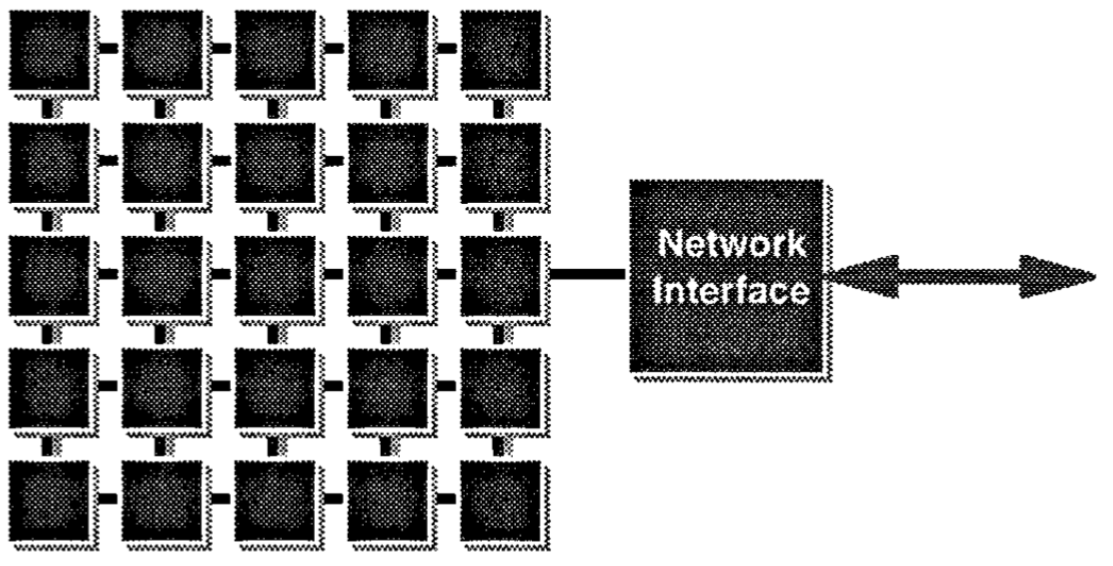
\includegraphics[width=0.95\linewidth]{Figures/Rep4DistrMemSys.png}
	\caption{Connecting a distributed-memory system to a network., Source: \cite{steenkiste1997high}.} 
    \label{fig:rep4:conndistrmem}
\end{figure}

% \motive
% There is a bottleneck in communication on \acs{dmm} which needs to be reduced.

\objective
An I/O architecture is created that supports high-speed I/O using a simple network interface to solve this problem.

\summary
\Ac{dmm}s communicate through a network interface that is connected both to the external network and the internal interconnect of the system (see: \cref{fig:rep4:conndistrmem}).



% High speed I/O for \ac{dmm} is difficult because the system is designed to operate in a distributed fashion where serialization is avoided as much as possible.
It is hard to implement the following tasks on a \ac{dmm}: the communication protocol (does not parallelize well), resource scheduling, data collection (data is typically divided between the private memories of the individual nodes). 
These tasks roughly correspond to the OSI network model (see: \cref{fig:rep4:osi}).
Additional problems are that some \acs{dmm} have slower internal links than the high-speed local-area networks such as \ac{hippi}.
Furthermore, applications on \ac{dmm} have diverse I/O requirements.

\begin{figure}
    \centering
	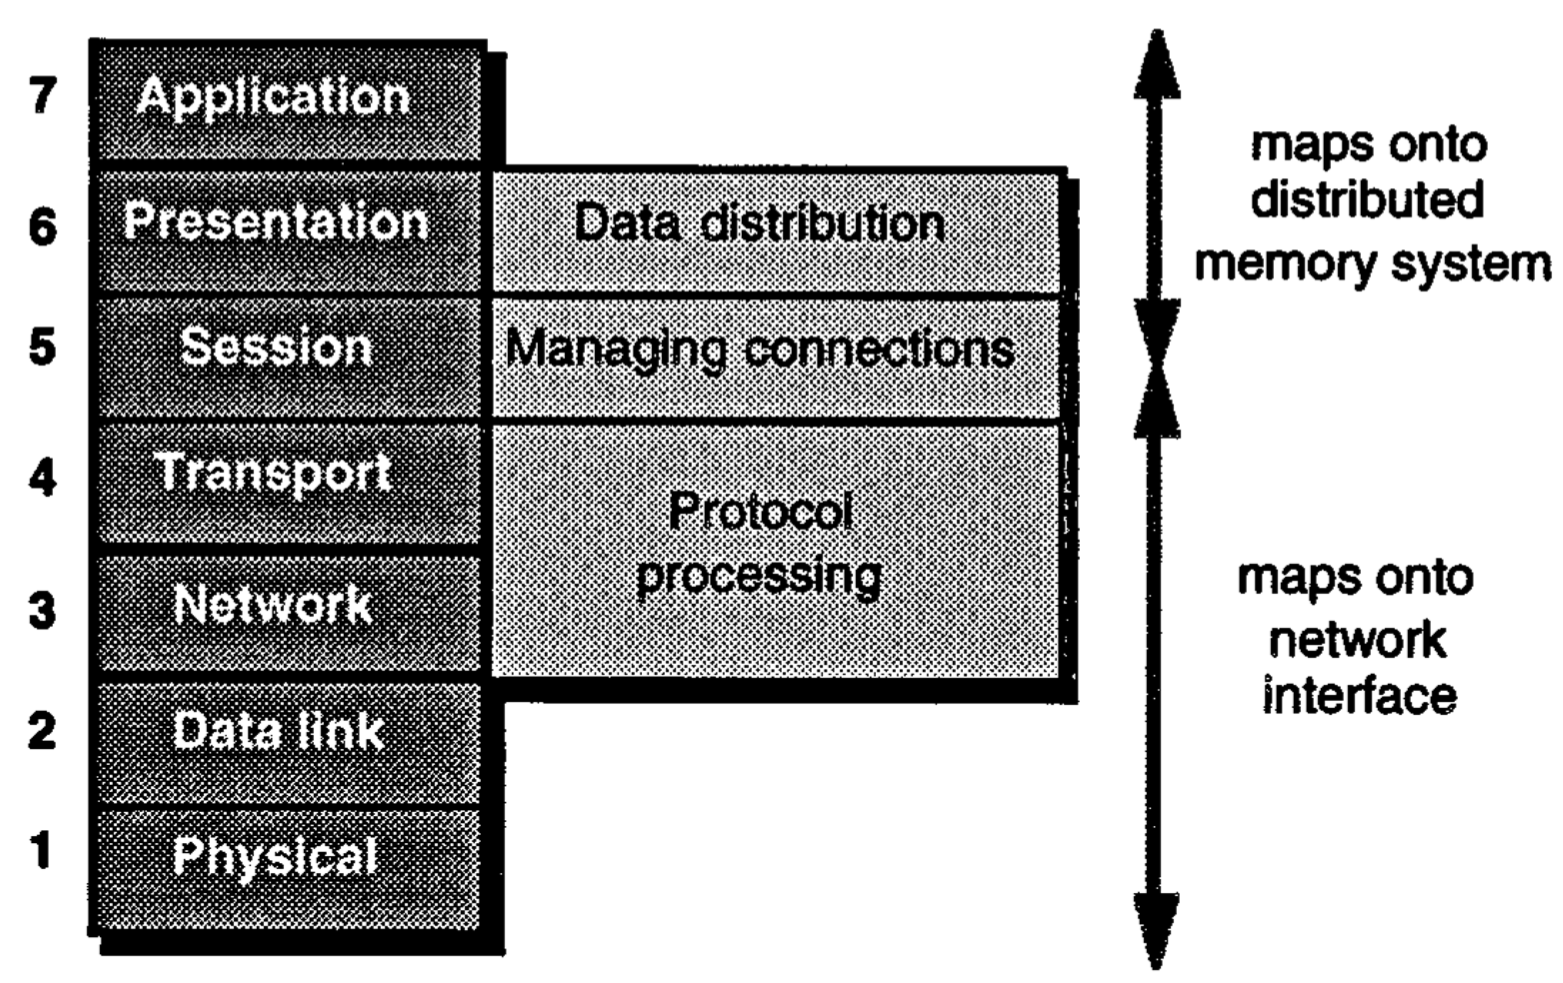
\includegraphics[width=0.95\linewidth]{Figures/Rep4OSI.png}
	\caption{Mapping of the protocol stack., Source: \cite{steenkiste1997high}.} 
    \label{fig:rep4:osi}
\end{figure}

%2.2 Architecture
\subsection{Architecture}
The designed I/O architecture allows the communication tasks to be performed on the \ac{dmm} as much as possible in combination with a network interface (\acc{hib}, see: \cref{fig:rep4:hib}).
The communication tasks are mapped in the following ways:
\begin{itemize}
    \item Processing of the transport and network protocol is performed on the (serial) network interface (\ac{hib}).
    \item The network interface provides an I/O interface that can be implemented efficiently on the network interface.
    \item The \ac{dmm} combines the distributed data on the private memories to large blocks for the network interface to process.
\end{itemize}

This mappings allows for appropriate scaling with network speed and data complexity.
This architecture is implemented for the iWarp system and a \ac{hippi} network.

%3 iWarp overview
\subsection{iWarp overview}
The iWarp system is a distributed-memory parallel computing system and combines high-speed computation and a communication agent in one component.
The communication agent connects an iWarp cell to four iWarp cell neighbours (see: \cref{fig:rep4:torus}).

\begin{figure}
    \centering
	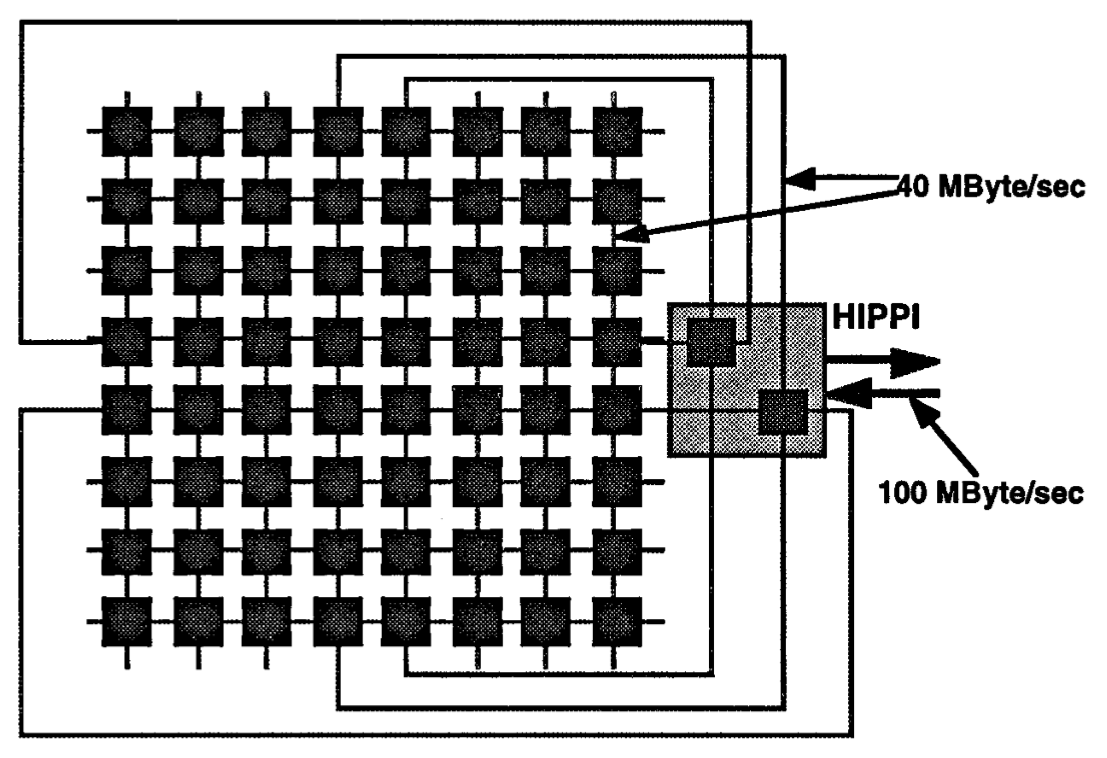
\includegraphics[width=0.95\linewidth]{Figures/Rep4torus.png}
	\caption{The \ac{hippi} network interface connected to the iWarp \ac{dmm}, also called the \textit{torus}., Source: \cite{steenkiste1997high}.} 
    \label{fig:rep4:torus}
\end{figure}

iWarp systems communicate with their external environment through I/O nodes linked to the torus (see: \cref{fig:rep4:torus}).
Applications produce output by sending data over the internal interconnect to the I/O node.

%4. Transport protocol processing
\subsection{Transport protocol processing}
Protocol processing is an potential bottleneck in network communication, it is inherently sequential.
There are two general categories in which protocol processing can be divided: overhead associated with every packed sent and overhead that scales with the number of bytes.
The latter will dominate as networks get faster.
The solution lies in making these operations efficient by minimizing the number of times the data is touched.

%4.2 network interface architeutre
\begin{figure}
    \centering
	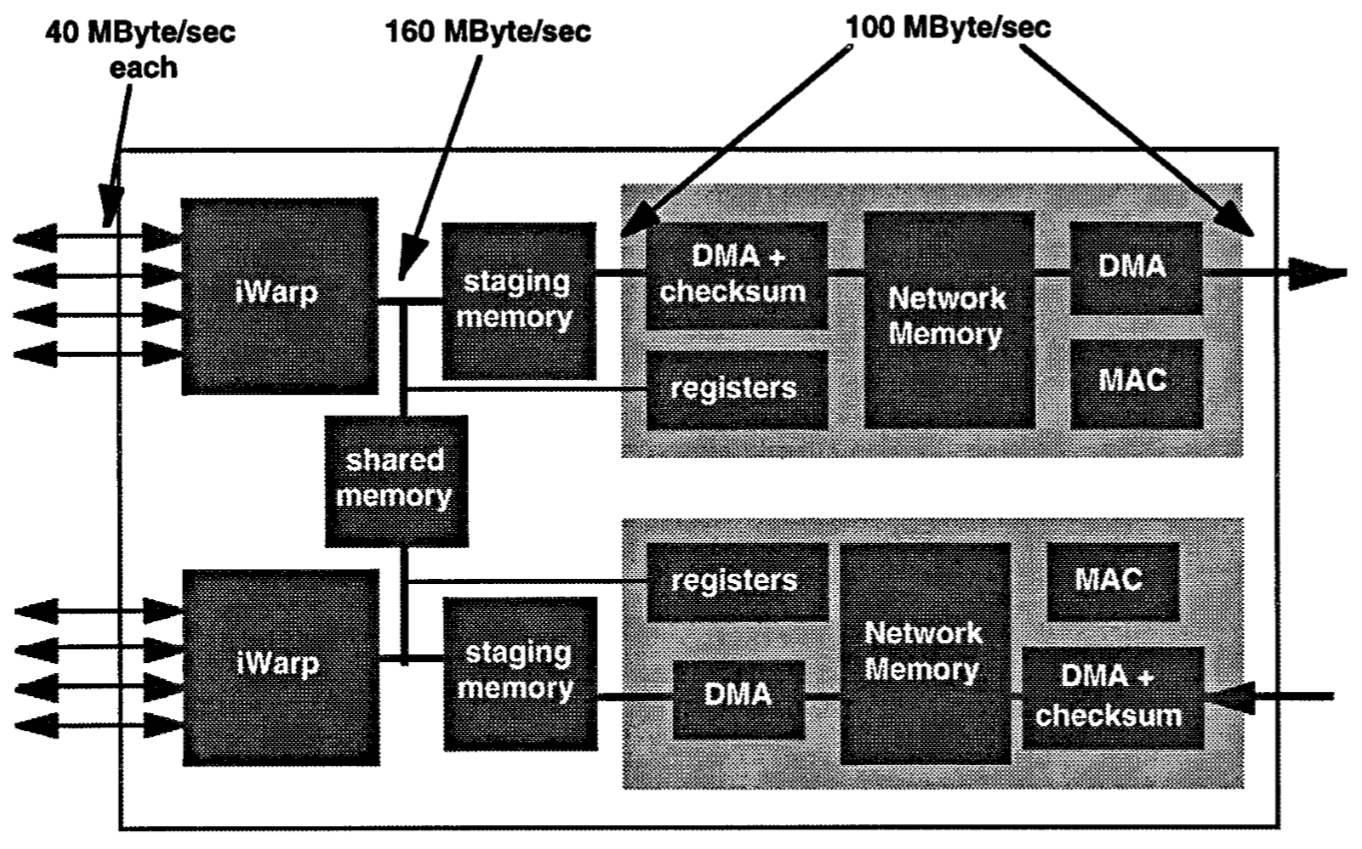
\includegraphics[width=0.95\linewidth]{Figures/Rep4hib.png}
	\caption{The \ac{hippi} interface Board Architecture. The gray areas show the communication acceleration blocks, Source: \cite{steenkiste1997high}.}
    \label{fig:rep4:hib}
\end{figure}

In \cref{fig:rep4:hib} the \ac{hib} is shown.
In the architecture the iWarp processor is responsible for per-packet operations, while the \acc{cab}, highlighted in the gray areas, is responsible for the per-byte operations.
%MS: missing connection with the CAB here
The high-bandwidth requirements typically make the memory bus the bottleneck of the network interface (\ac{hib}).
The \ac{hib} uses a couple of mechanisms to optimize the memory bandwidth utilization: it uses two iWarp processors (doubling of memory bandwidth) and the \ac{hib} uses two levels of memory optimized for different types of accesses.

% %Could have written something about 4.3 protocol software
% Measurement for raw \ac{hippi} and UDP over IP gave the same throughput results establishing that the UPD/IP implementation is very efficient.

% 5. THE STREAMS I/O ARCHITECTURE
\subsection{Stream I/O architecture}
There are two phases in which the transfer of data happens: the data is transferred from the distributed-memory system to the network interface and in the second phase data is transferred to the network.
Managing the first phase is a resource management problem which is tackled with the stream architecture (see: \cref{fig:rep4:streams}).

\begin{figure}
    \centering
	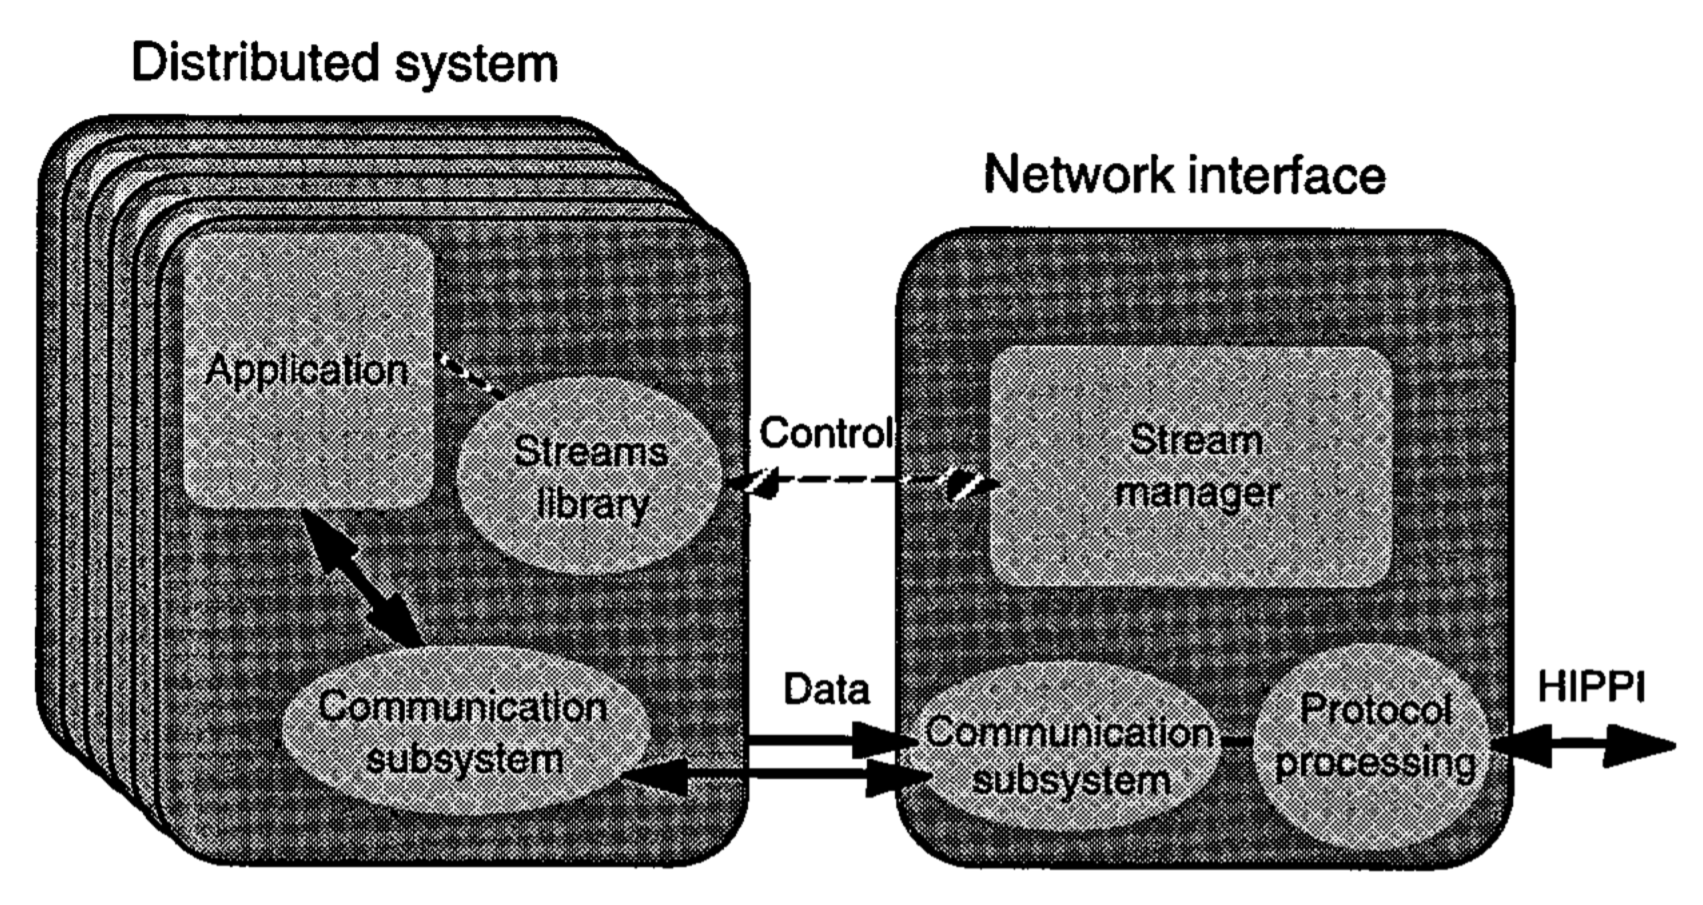
\includegraphics[width=0.95\linewidth]{Figures/Rep4streamsarchitecture.png}
	\caption{The stream architecture., Source: \cite{steenkiste1997high}.}
    \label{fig:rep4:streams}
\end{figure}

It is based on logical connections, each one supporting communication between the application on a \ac{dmm} to a destination on the external network.
A stream is defined as a data transfer on an established connection.
The application on the \ac{dmm} is responsible for distribution of the data to the network interface (\ac{hib}).
The \textit{stream manager} on the network interface is responsible for efficient data movement of multiple streams.

%5.2 dataformat
In the stream architecture the application provides the stream manager with information regarding the data format. 
This way the stream manager can plan and optimize the data transfers.

%5.3 iWarp streams software

%6. Data reshuffling in support of high-speed I/O
\subsection{Reshuffling}
Utilizing large number of processors allows for data parallelism.
The data throughput depends on the number of links (due to striping) and the total message size.
Using data reshuffle, the throughput is optimized for different applications.

The \ac{dmm} is used for the scatter/gather operation.
This allows for the interface  node only to deal with large blocks of data and minimizes the cost on the network interface.

Also, reshuffling is an easy to parallelize operation which enables efficient reshuffle.
Parallelizing compilers have enough information to map a program onto a \ac{dmm} and provide it with the appropriate calls to do reshuffling.

%Conclusion
\subsection{Conclusion}
An architecture for network I/O is presented on \acs{dmm} and fast I/O rates over the iWarp \ac{hippi} interface were enabled.
This throughput was possible by a couple of key features: offloading of application specific tasks to the \ac{dmm}, the stream manager optimizes the network resource management.




%%%%%%%%%%%%%%%%%%%%%%%%%%% 1  %%%%%%%%%%%%%%%%%%%%%%%%%%%
\section{An 8 x times,5 Gb/s Parallel Receiver With Collaborative Timing Recovery \cite{agrawal20098}}  \label{ss:agrawal20098}
%%%%%%%%%%%%%%%%%%%%%%%%%%% 1  %%%%%%%%%%%%%%%%%%%%%%%%%%%

Clock frequencies have been increasing in the early part of the century up to a certain point.
To alleviate bottle-necks in the performance of a system the \textit{off-chip} input and output (I/O) should also be scaled.
Scaling of \acc{bw} is obviously achievable by implementation of parallel I/O.
Digital systems need a clock signal for operation.
Nowadays, digital systems are relatively large \footnote{more parallel I/O leads to a larger system.} and this gives problems in synchronicity of digital systems.
To correct for this, timing recovery (or symbol synchronization \cite{mueller1976timing}) is applied.
Parallel links are conventionally implemented as \acc{embeddedlink} (see: \cref{fig:rep1:seriallinks}) or as \acc{synclink}  (see: \cref{fig:rep1:synclinks}).

\begin{figure}	\centering
	
	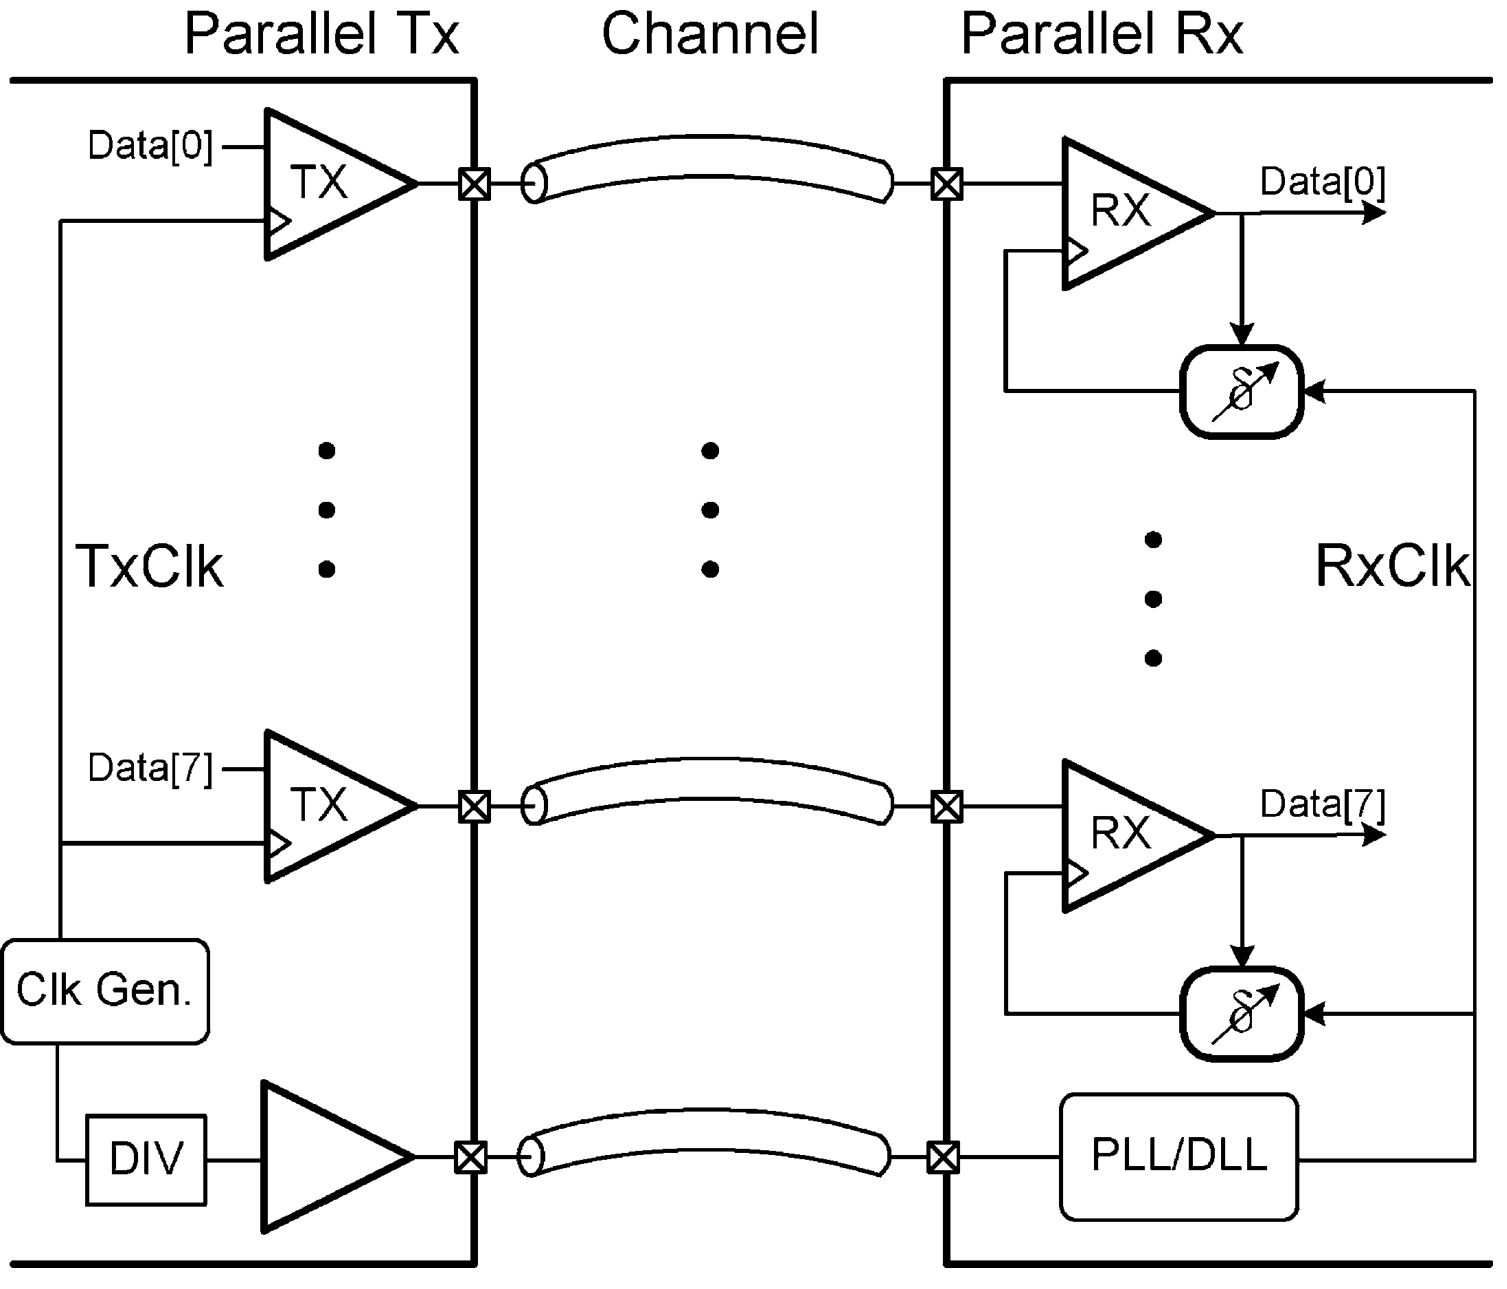
\includegraphics[width=0.8\linewidth]{Figures/Rep1SourceSync.png}
	\caption{Ensemble of serial links (\textit{embedded clock link}) (\ac{embeddedlink}), Source: \cite{agrawal20098}.} 
    \label{fig:rep1:seriallinks}
\end{figure}

\begin{figure}	
    \centering
	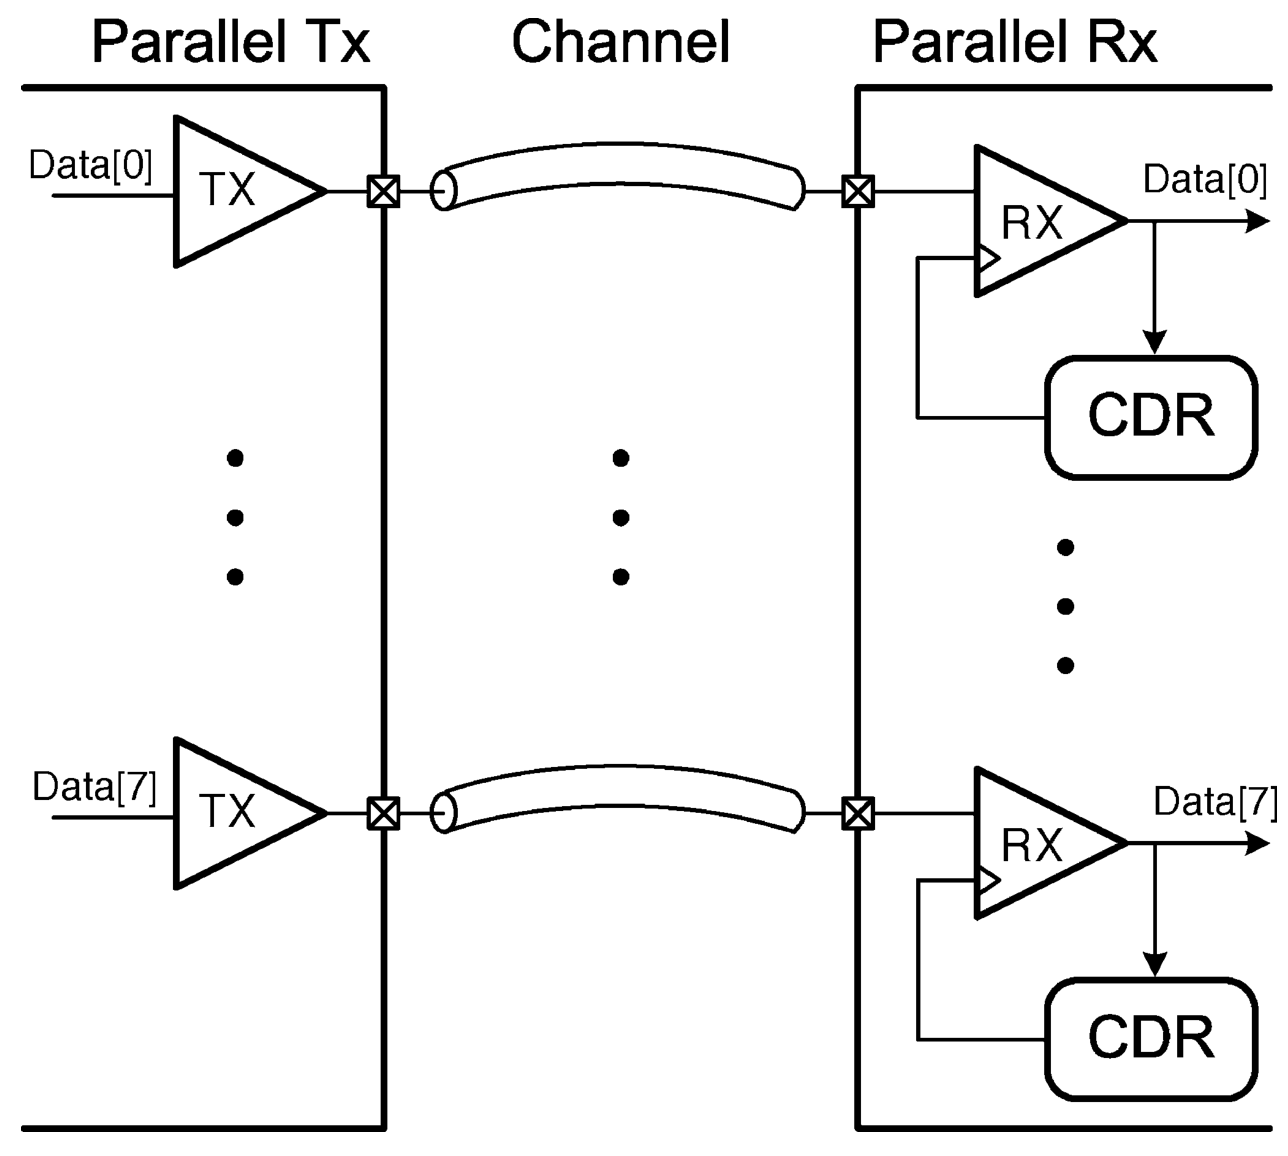
\includegraphics[width=0.8\linewidth]{Figures/Rep1EnsembleSerLinks.png}
	\caption{Source-synchronous links (\textit{forwarded-clock link}) (\ac{synclink}), Source: \cite{agrawal20098}.} 
    \label{fig:rep1:synclinks}
\end{figure}

In \ac{embeddedlink} the receiver extracts the clock from the data, as it is embedded in the data. 
In \ac{synclink} a clock line is sent along the data and the receivers can use it for timing recovery. 
\objective
The increased I/O \ac{bw} puts a strain on the latency, power consumption and form-factor requirements and causes jitter amplication. 
\motive
The research aim of this paper is to merge the desirable characteristics of both \ac{embeddedlink} as \ac{synclink} into \acc{coltimrec}.
This design comes with an power and area overhead of 10-15\% relative to \ac{synclink} but is more efficient than the \ac{embeddedlink} and also increases the effective edge transition density.
% \footnote{This concept is more clearly explained in \cite{miller2005transition}}.
\summary
The design of the \ac{coltimrec} is shown in \cref{fig:rep1:coltimrec}. 
It does not contain a clock link (as in \ac{synclink}) and instead of a local \acc{cdr} as seen in \cref{fig:rep1:seriallinks} the local clock data is connected to a \acl{gtr} block (\ac{gtr}) which carries the responsibility of the providing the global clock.

\begin{figure}
    \centering
	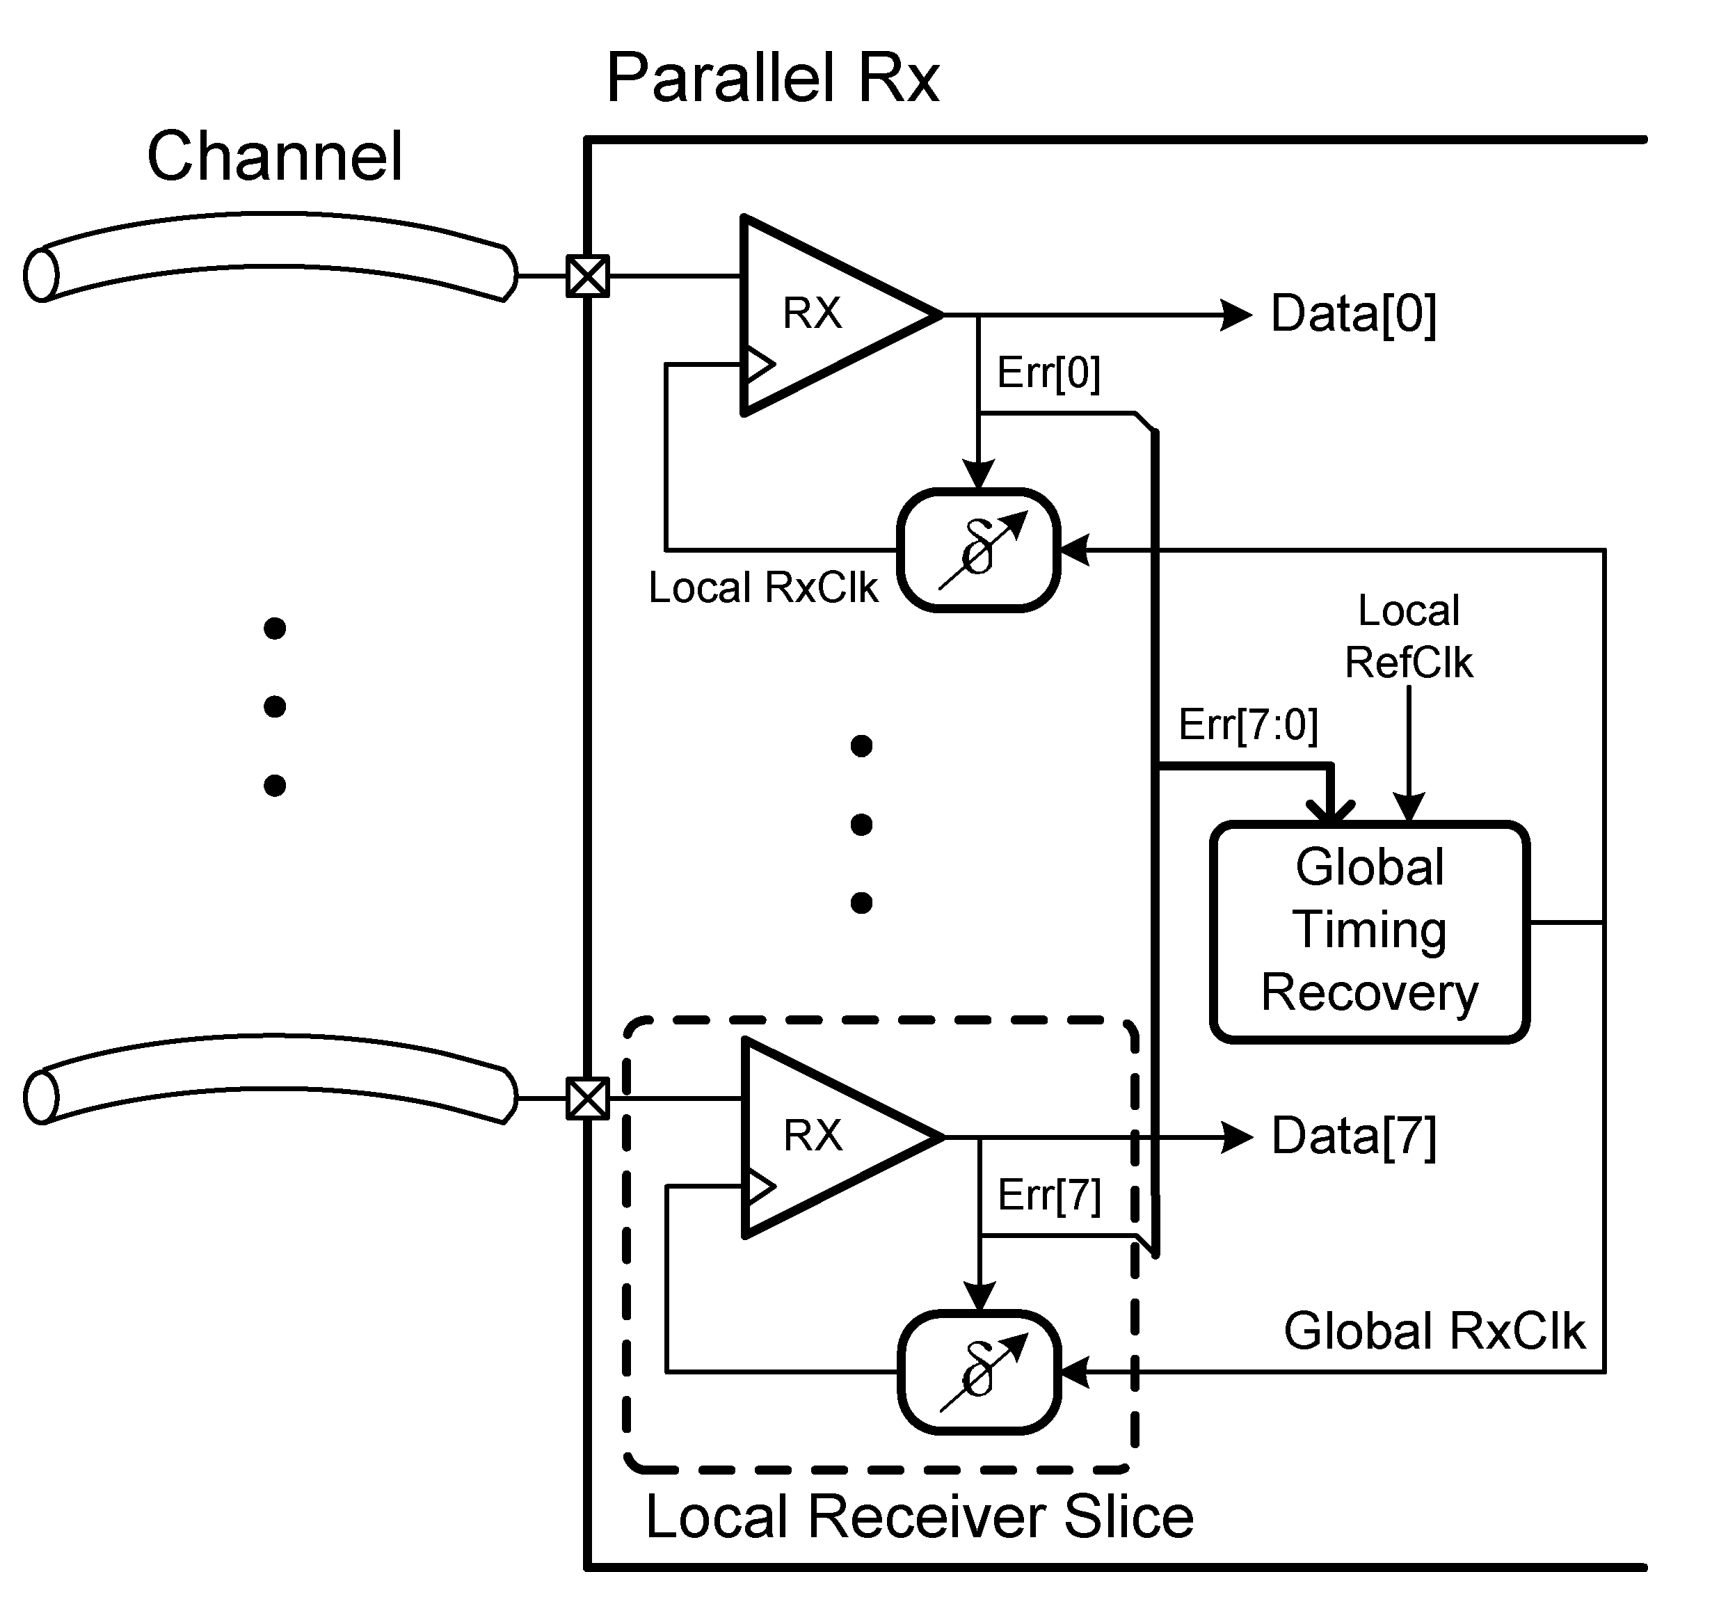
\includegraphics[width=0.85\linewidth]{Figures/Rep1CombLink.png}
	\caption{\acc{coltimrec}, Source: \cite{agrawal20098}.} 
    \label{fig:rep1:coltimrec}
\end{figure}

A comparison has been made between three different levels of jitter scenarios regarding phase-tracking error for each system (\ac{embeddedlink}, \ac{synclink} and \ac{coltimrec}). %\footnote{Jitter: the deviation from periodicity, it is a form of noise. Dither on the other hand is intentional noise in an out of band frequency.} 
The noise levels are devided in the following way: low-frequency jitter (around 1 MHz), midfrequency jitter (around 30 MHz) and high-frequency jitter (around 1 GHz).
Phase tracking at low-frequency jitter is best for \ac{embeddedlink}. 
At mid-frequency jitter the \ac{coltimrec} behaves much better than the other implementations. 
At high-frequency jitter all systems behave poorly.
However, trends show that mid-frequency jitter is growing, which motivates \ac{coltimrec}.

The design of the \ac{coltimrec} (\cref{fig:rep1:coltimrec}) consist of two global parts: the phase adjustment element and the \acc{gtr} block.
Each local receiver sends early/late timing information to the \ac{gtr}.
The \ac{gtr} sends the recovered clock (Global RxClk) that tracks the frequency and the jitter of the data signals.
% \footnote{Skew: the possible difference in arrival time of the clock in different sections of a design} 
To handle the interchannel skew the local receivers alter the phase of the Global RxClk for inter-channel skew.

% Explain the GLOBAL working of the global timing recovery circuit
The \ac{gtr} is comprised of an Error retimer, phase error summer, $2^{nd}$ order filter, \acc{pll} and a phase interpolator.
The error retimer aligns the clock of 8 channels to a reference clock.
The phase error summer, sums the phase error of the 8 channels and passes it to the filter.
The filter delivers the decoded information to the \ac{pll} and the phase interpolator.
The \ac{pll} receives the filter information and uses it to select odd and even phase difference (2 4b-muxes).
This is coarse grained phase generation.
The phase interpolator provides a 256 phase steps per clock period delivery (more fine grained phase adjustment).
% Explain the GLOBAL working of the phase adjustment element
The phase adjustment consists of two \accs{dll}, data sampler (8 channels), duty-cycle corrector, skew-compensation element and a phase spacing error correction circuit (see: \cref{fig:rep1:receiver}).
The global clock (from the \ac{gtr}) is corrected for its duty-cycle.
The first \ac{dll} provides phase de-skewing for phase alignment of its local clock and the data.
The second \ac{dll} generates 8 uniformly spaced clock phases to drive the interleaved data samplers.
%not clear why
Reasons for using the cascaded \acsp{dll} approach are: \acsp{dll} do not limit the global TR \ac{bw} and they require only one phase to generate a local clock.
However, the two \acsp{dll} could be replaced by one \ac{pll}.
This was not applied because \acsp{dll} do not apply phase filtering. 
But there are disadvantages to \acsp{dll} that should taken into account.
For instance, \acsp{dll} are very sensitive to the duty cycle of the reference clock and the shape of the reference clock can amplify a mismatch in phase spacing.

\begin{figure}	
    \centering
	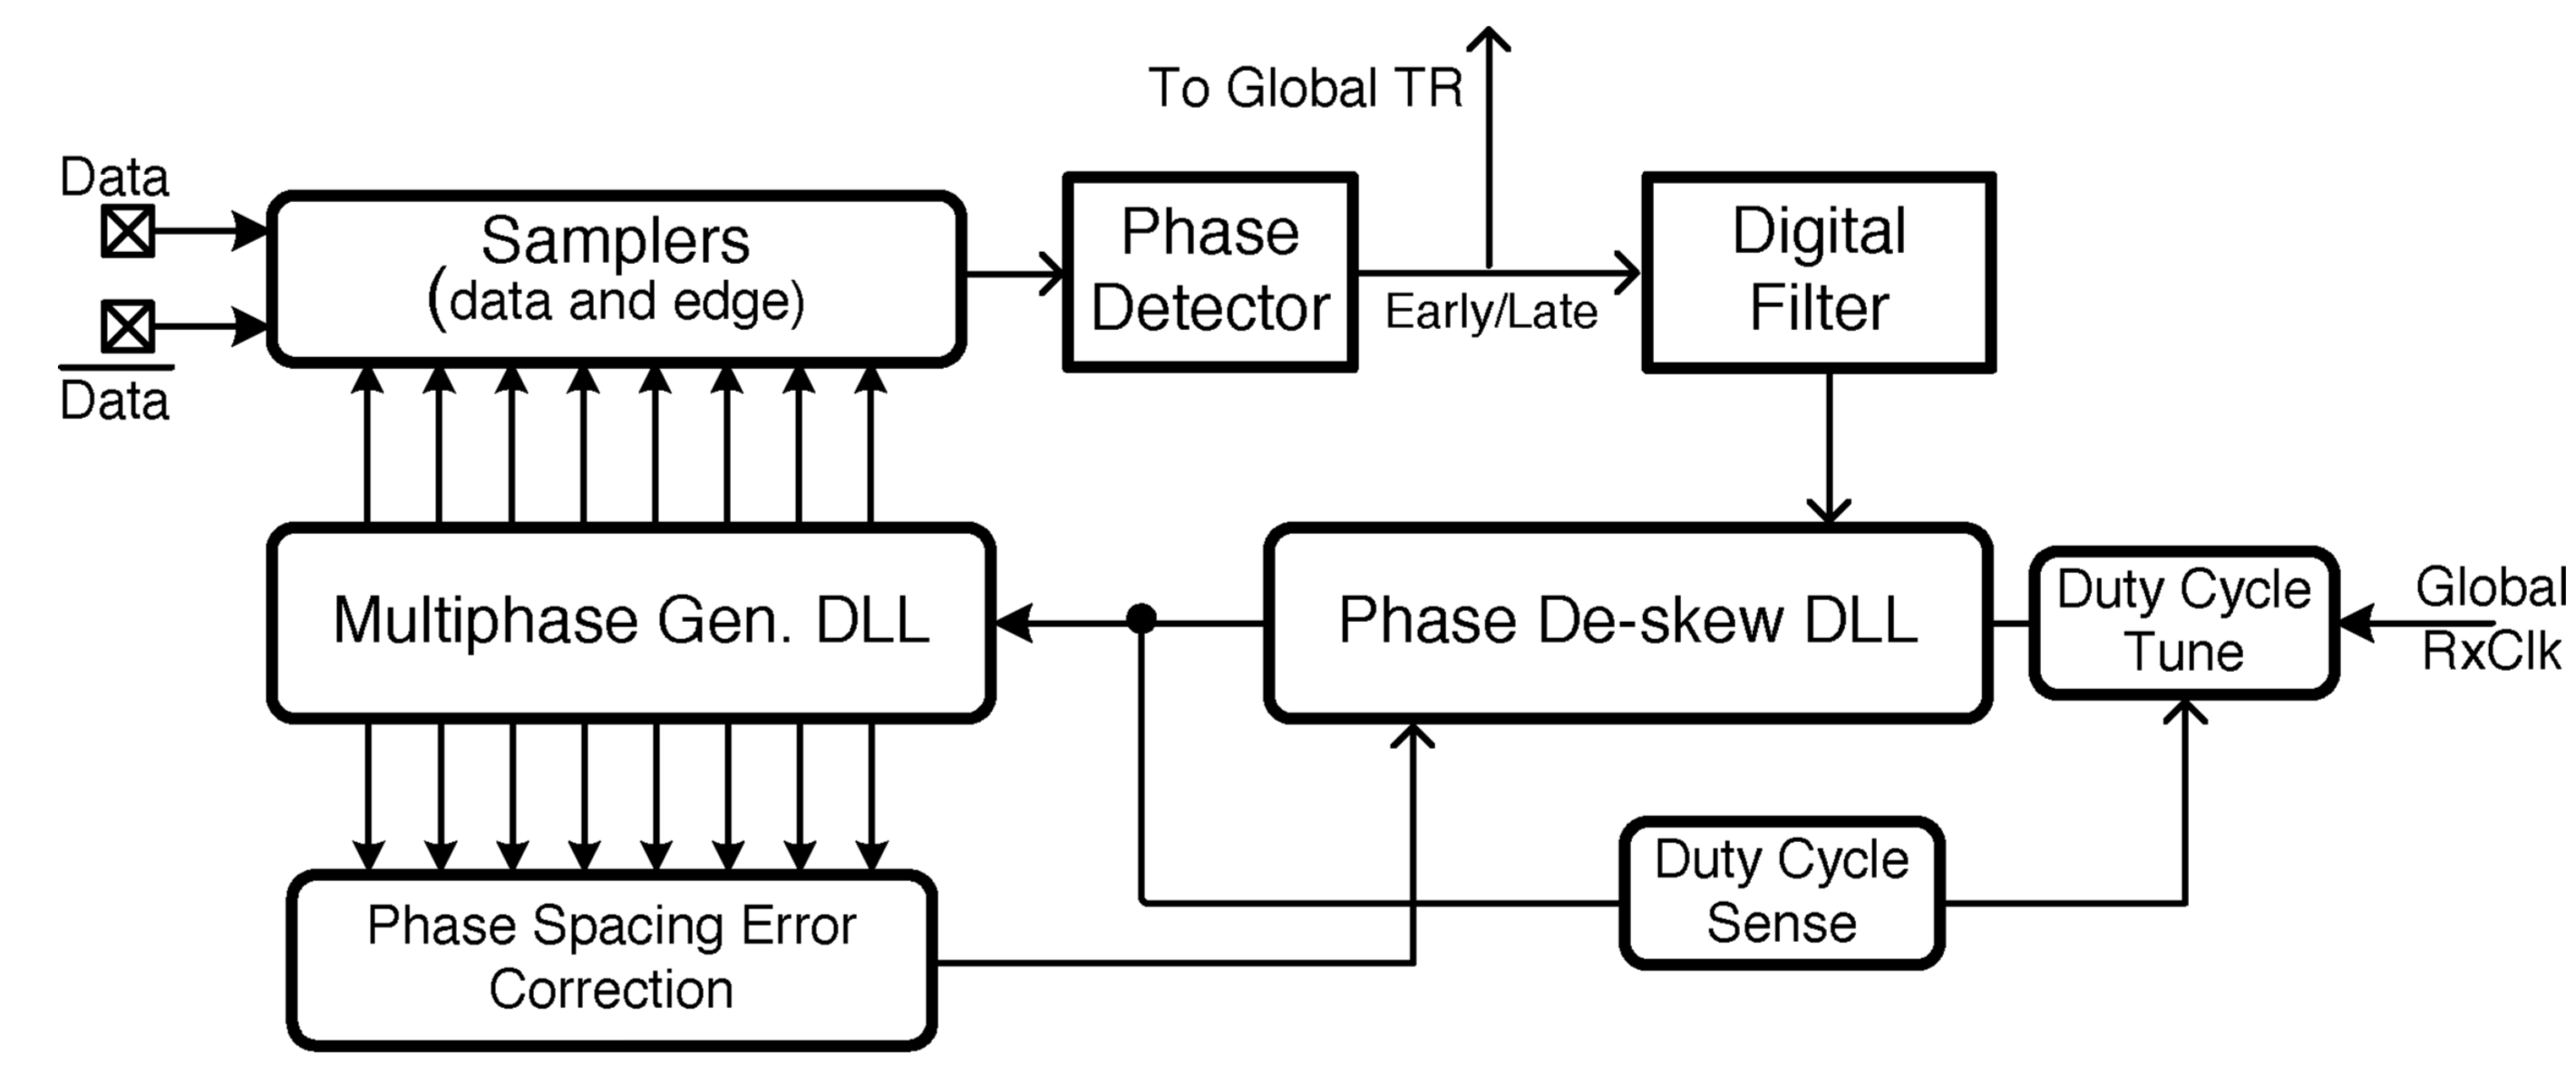
\includegraphics[width=0.99\linewidth]{Figures/Rep1ReceiverSlice.png}
	\caption{Local receiver slice block diagram, Source: \cite{agrawal20098}.} 
    \label{fig:rep1:receiver}
\end{figure}
% Measurements and results
The setup was tested on 130 nm CMOS logic. 
To test the chip 8 synchronous PRBS data signals are needed which also add amounts of correlated jitter.
This was done by using a Tektronix 5334 up to 3.2 Gb/s.
For the higher rates an FPGA based parallel transmitter was used.
Not all channels were tested due to restricted connector spacing on the board .

\Cref{fig:rep1:result} shows the dithering jitter on the recovered clock. 
When the number of channels share timing information the dithering jitter reduces from 2.7ps to 2.2ps.

% Discussion / conlusion
Wideband jitter tracking, by reducing dithering jitter on the received clock, is possible when implementing \ac{coltimrec} however there is an area and power overhead (respectively 8.5\% and 15\% per receiver).

\begin{figure}	\centering
	
	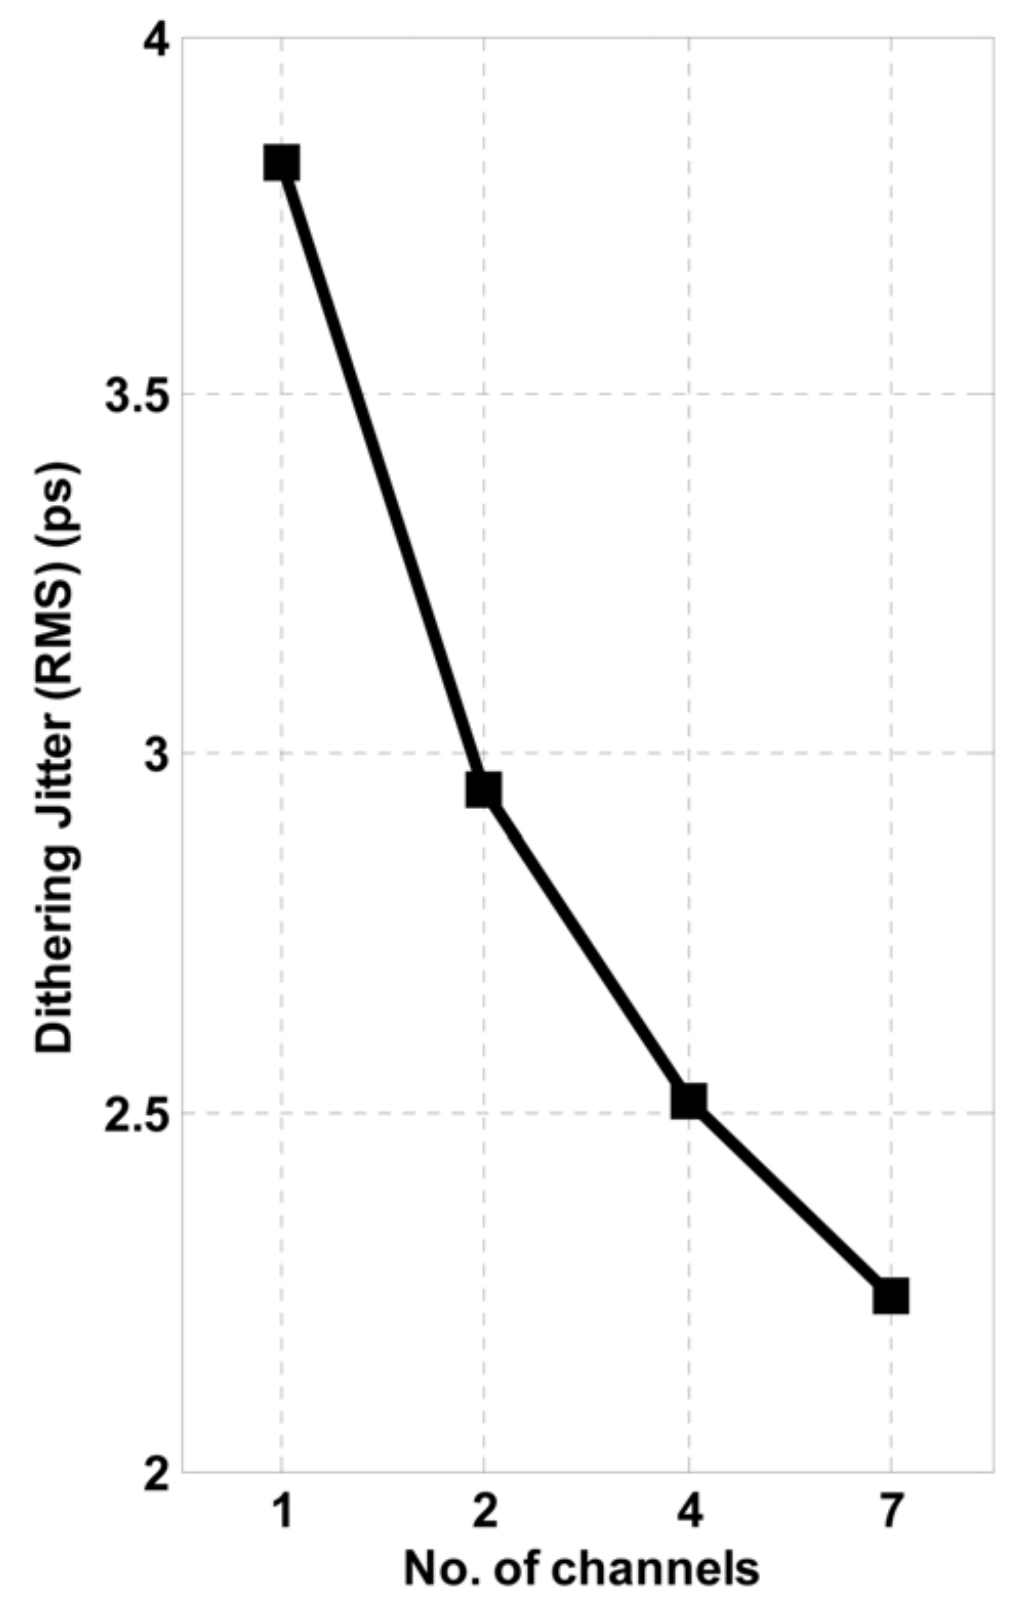
\includegraphics[width=0.7\linewidth]{Figures/Rep1Result.png}
	\caption{Measured RMS jitter for different degrees of collaboration, Source: \cite{agrawal20098}.} 
    \label{fig:rep1:result}
\end{figure}

% Motive: Statement indicating why the research was done (e.g. a gap in
% knowledge, contradictory results). The motive leads to the objective.
% • Objective: Statement about what the authors want to know. The
% objective may be formulated as a research question, a research aim, or a
% hypothesis that needs to be tested.
% • Main conclusion: Statement about the main outcome of the research. The
% main conclusion is closely connected to the objective. It answers the
% research question, it says whether the research aim was achieved, or it
% states whether the hypothesis was supported by evidence.

% In the body, you should:
% - Group research studies and other types of literature (reviews, theoretical articles, case studies, etc.) according to common denominators such as qualitative versus quantitative approaches, conclusions of authors, specific purpose or objective, chronology, etc.
% - Summarize individual studies or articles with as much or as little detail as each merits according to its comparative importance in the literature, remembering that space (length) denotes significance.
% - Provide the reader with strong "umbrella" sentences at beginnings of paragraphs, "signposts" throughout, and brief "so what" summary sentences at intermediate points in the review to aid in understanding comparisons and analyses.



%%%%%%%%%%%%%%%%%%%%%%%%%%%  2  %%%%%%%%%%%%%%%%%%%%%%%%%%%
\subsection{Low-power, high-speed transceivers for network-on-chip
communication \cite{schinkel2009low}} \label{ss:schinkel2009low}
%%%%%%%%%%%%%%%%%%%%%%%%%%%  2  %%%%%%%%%%%%%%%%%%%%%%%%%%%
The interconnect of a chip has become a bottleneck regarding speed, power en reliability of chip due to its high capacitance and high resistance. \acc{noc} technology is a good candidate for future progress.
\ac{noc} is for instance more power efficient and allows for different kinds of synchronous and asynchronous techniques.

% IETS ZEGGEN OVER TOEGEPASTE TECHNOLOGIE

\motive
However, when using \acsp{noc} still a lot of power is consumed.
For instance, the on-chip network consumes $39\%$ of the total chip power is consumed \cite{vangal20075}.
It is proposed that a \ac{noc} can benefit from advanced \textit{link-transceivers}.

\objective
In this paper earlier proposed techniques by the authors (\cite{mensink20070}) to decrease the power consumption and to increase the data-rate are applied to \ac{noc} applications.
Tests show a reduced link power of 3.3 times and an increased the data-rate of 80\%.

\summary
In the process of applying the aforementioned optimization's some simplifying assumptions were made. 
For instance, a wire length of 2mm is assumed everywhere. 
The receiver equalization is omitted.

\begin{figure}[]
	\centering
	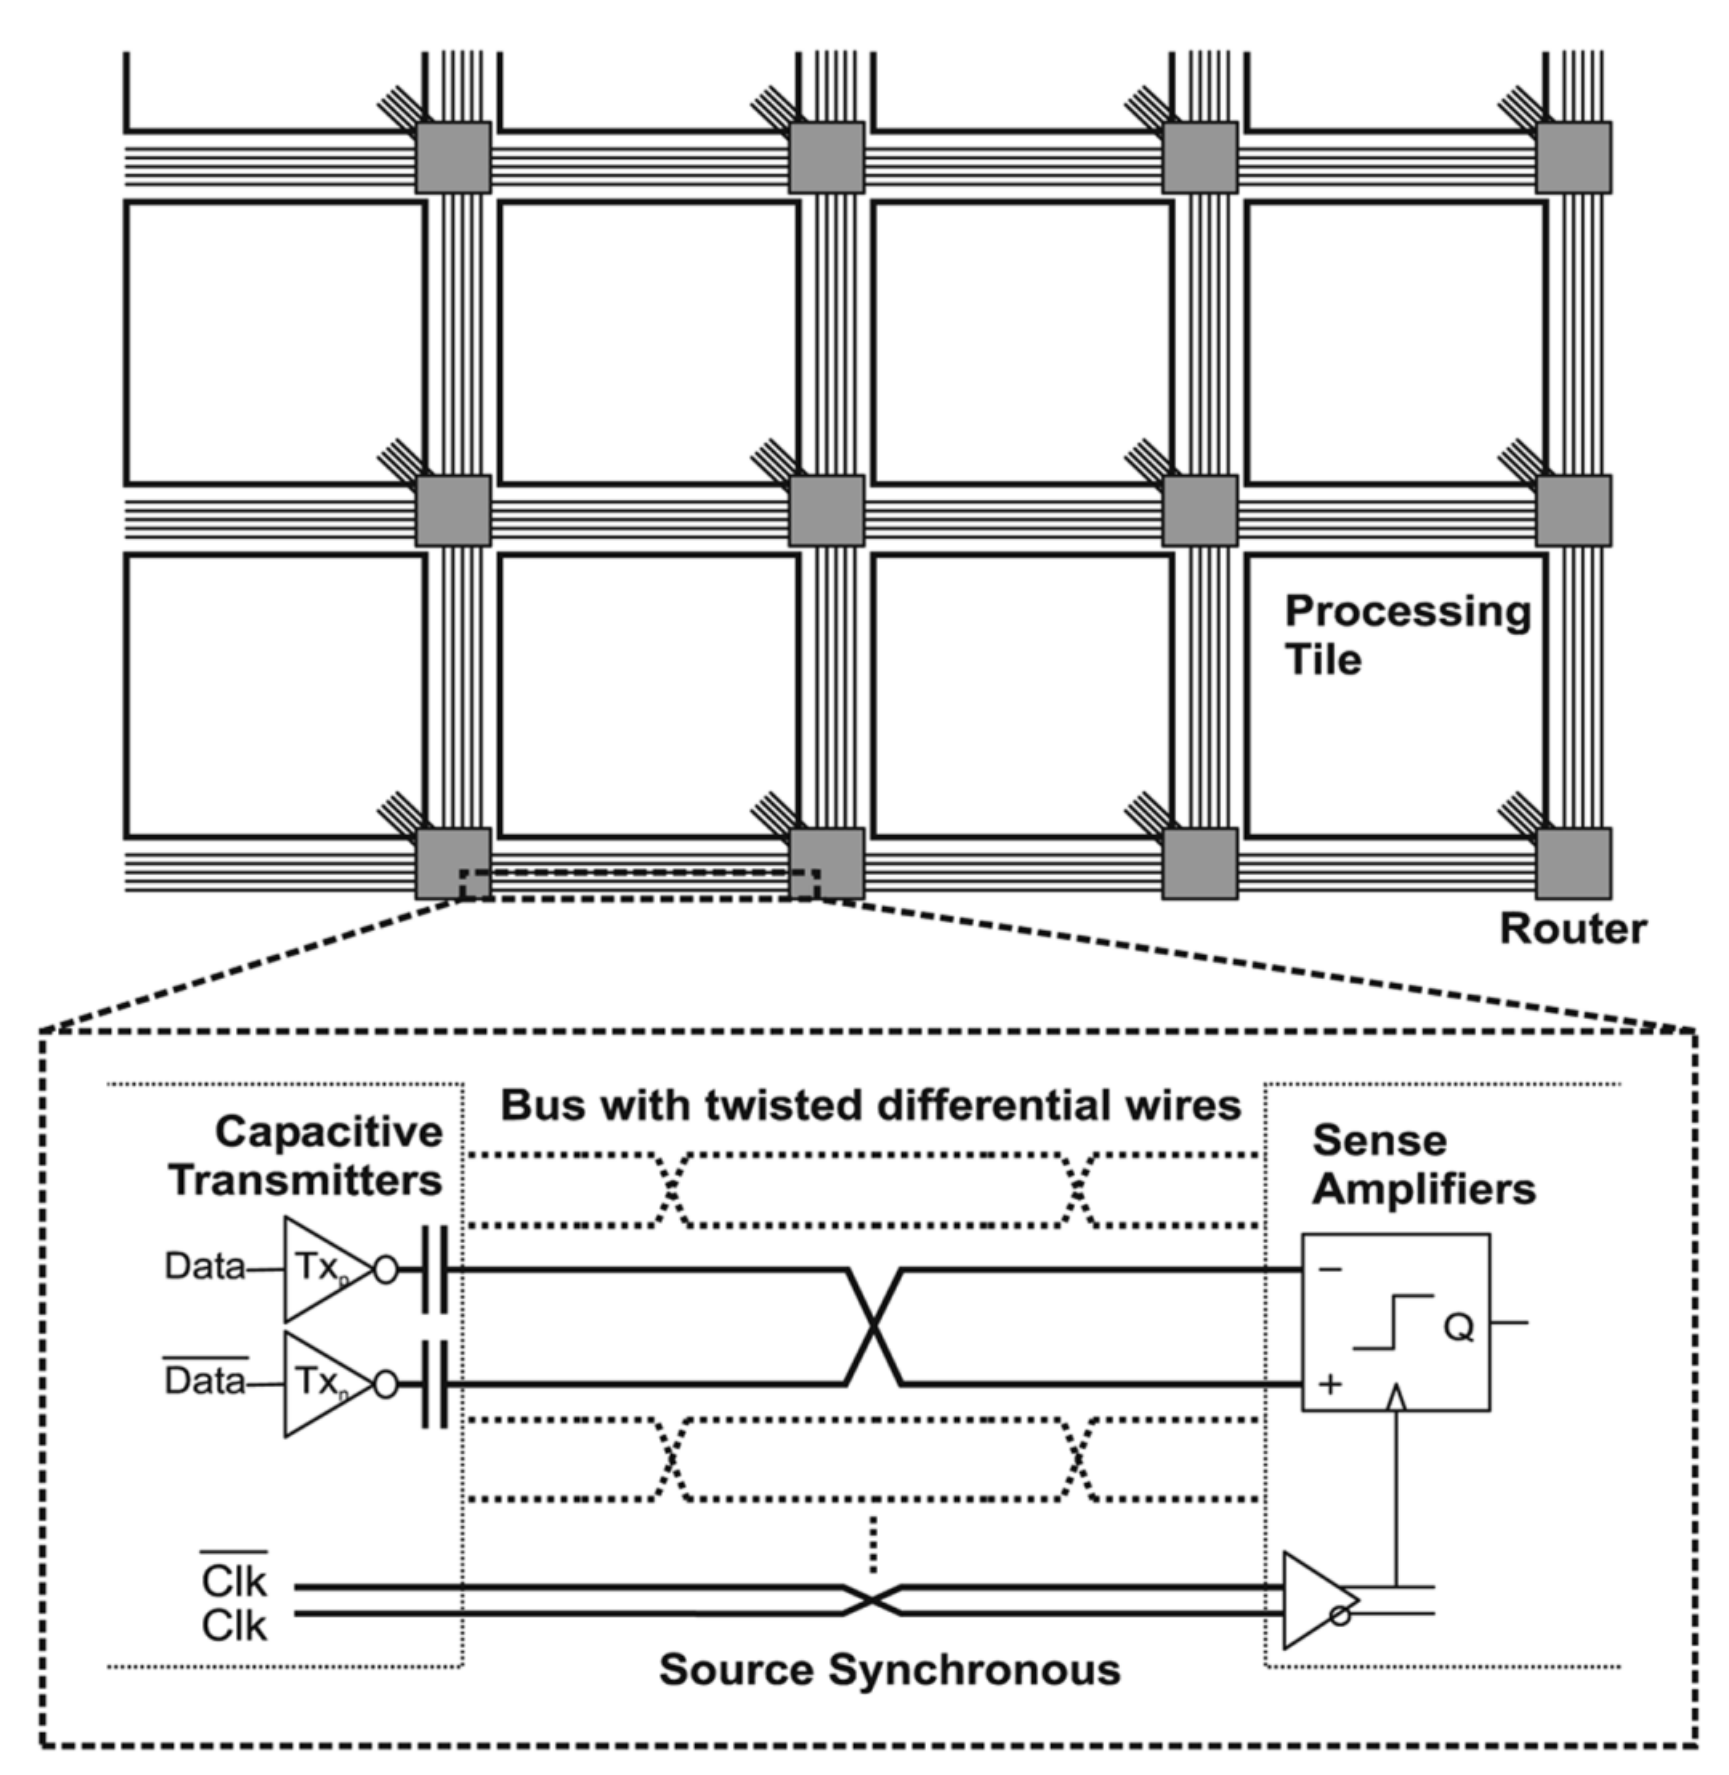
\includegraphics[width=0.78\linewidth]{Figures/Rep2Overview.png}
	\caption{Overview of the proposed transceiver for \acsp{noc}, Source: \cite{schinkel2009low}.} 
    \label{fig:rep2:overview}
\end{figure}

It is also assumed that the interconnects are unidirectional were bidirectional designs complication the design of fast transceivers.

The authors have implemented a set of optimization's which gave the improved performance:
\begin{itemize}
    \item The transmitters uses a series capacitance
    \item The interconnect consists of twisted pairs
    \item An improved sense amplifier
\end{itemize}


\subsubsection{Interconnect} \label{sss:rep2:interconnect}
Conventional transceivers are not suitable because its delay can vary due to crosstalk.
Crosstalk decreases the noise margin.
Standard technique to limit crosstalk is the use of shield-wires and shield-planes and to increase the spacing between wires.
For the highest possible data-rate the designer would place a shield-wire next to each signal wire.


Conventional transceivers would also need to (dis)charge large wire and driver capacitances.
A good way to reduce the power consumption is to use low-swing signaling (lower Vdd) but this reduces the noise margin.
Use of \textit{twisted differential wire} can reduce crosstalk and allow for lower power consumption. 
The increase in area and power is relatively small, because shield-wires are not necessary anymore.
However, a sensitive differential sense amplifier is needed with a high power-supply rejection and that can reliably operate at low noise margins (see: \cref{sss:rep2:senseamp}).

The use of twisted differential wires can mitigate crosstalk only needing one twist in an even pair and two twists in an odd pair \cite{mensink2007optimal}.


\subsubsection{Transmitter}
% As can be seen in \cref{fig:rep2:overview}
Because the link power has a significant part in the total power usage, it is desirable to reduce the link power. 
This is for instance achieved by implemented active circuits that allow for switching between High signal swing ($V_{DDH}$) and Low signal swing ($V_{DDL}$) called a Multi-$V_{DD}$ low-swing. 
However, these circuits come with their drawback. 
For instance, the noise-margin is directly related to the power supply noise. 
A short dip in one of the two supplies could introduce a bit-error.
Also, large transistors are needed to drive the interconnects with sufficient speed.
\\
The authors propose a capacitive pre-emphasis transmitter. 
A series capacitance $C_{TX}$ is used to drive the interconnect (see: \cref{fig:rep2:overview}). 
This capacitor acts as a capacitive divider which reduces a capacitive related swing by $C_{TX} / ( C_{WIRE} + C_{TX})$ and increases the bandwidth as $C_{TX}$ gives each transition an overshoot see: \cref{fig:rep2:capovershoot}.
Also, $C_{TX}$ attenuates the supply noise in comparison to low-swing transmitters.

\begin{figure}[]
	\centering
	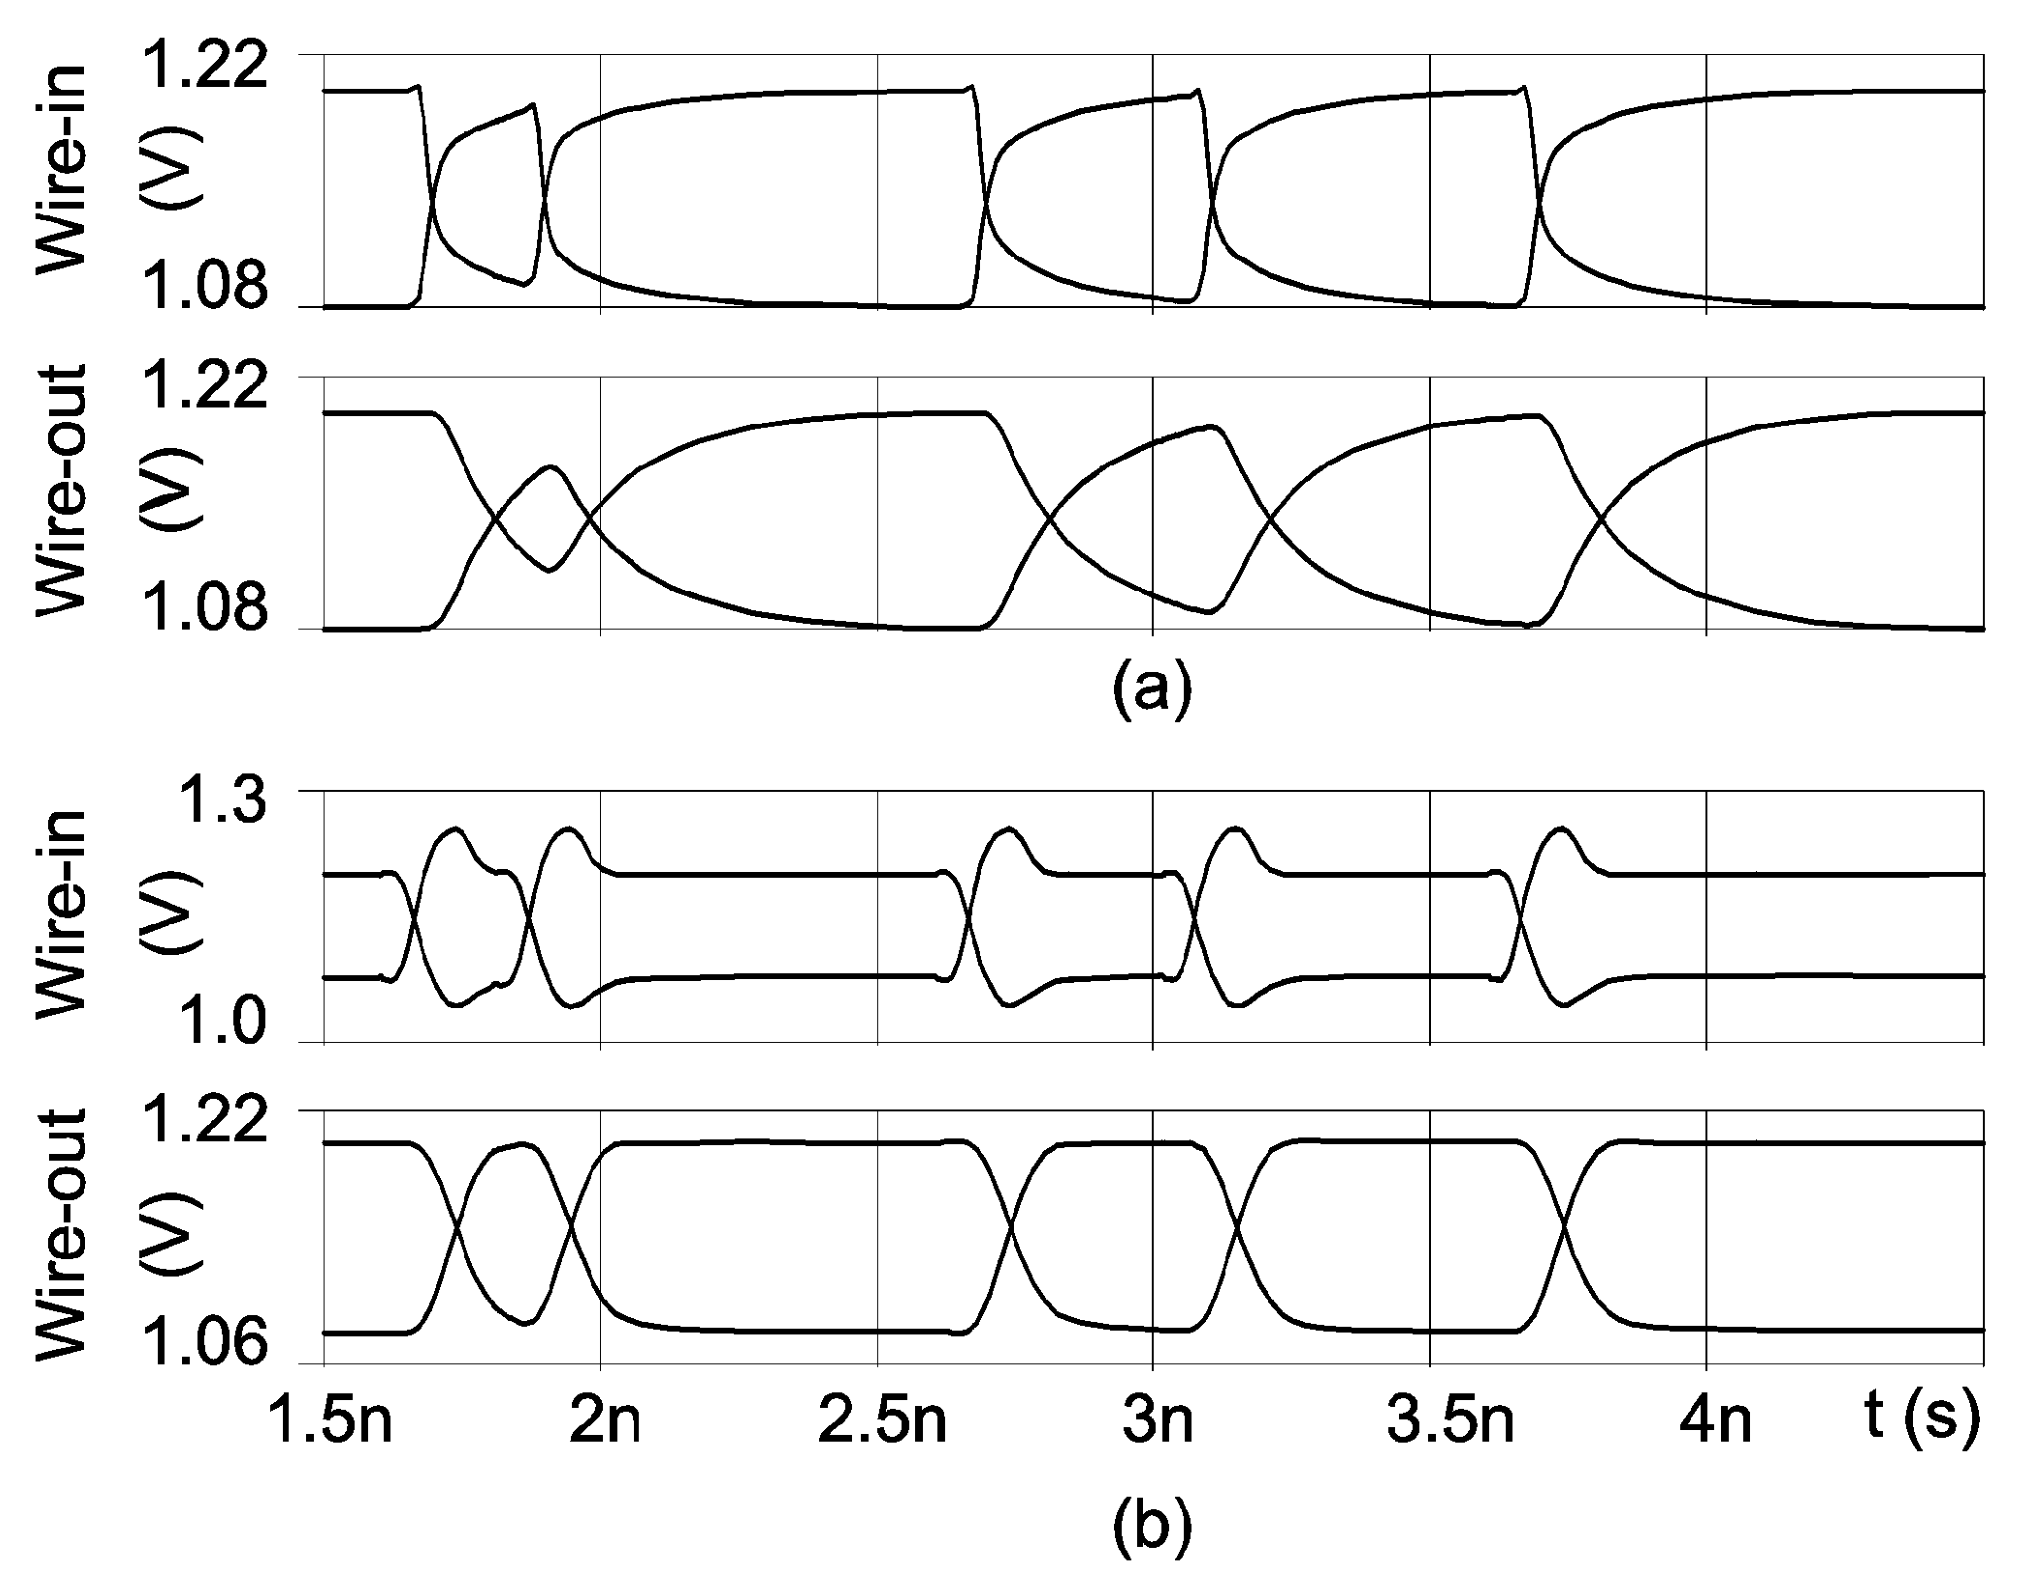
\includegraphics[width=0.8\linewidth]{Figures/Rep2TransmitterCap.png}
	\caption{Behaviour comparison of conventional transmitter (a) and a capactive transmitter (b), Source: \cite{schinkel2009low}.} 
    \label{fig:rep2:capovershoot}
\end{figure}

The capacitive transmitter has a 25 fJ overhead were a Multi-$V_{DD}$ low-swing setup uses 127 fJ per swing.



\subsubsection{Sense amplifier} \label{sss:rep2:senseamp} %IV Receiver and optimal swing

\begin{figure}[]
	\centering
	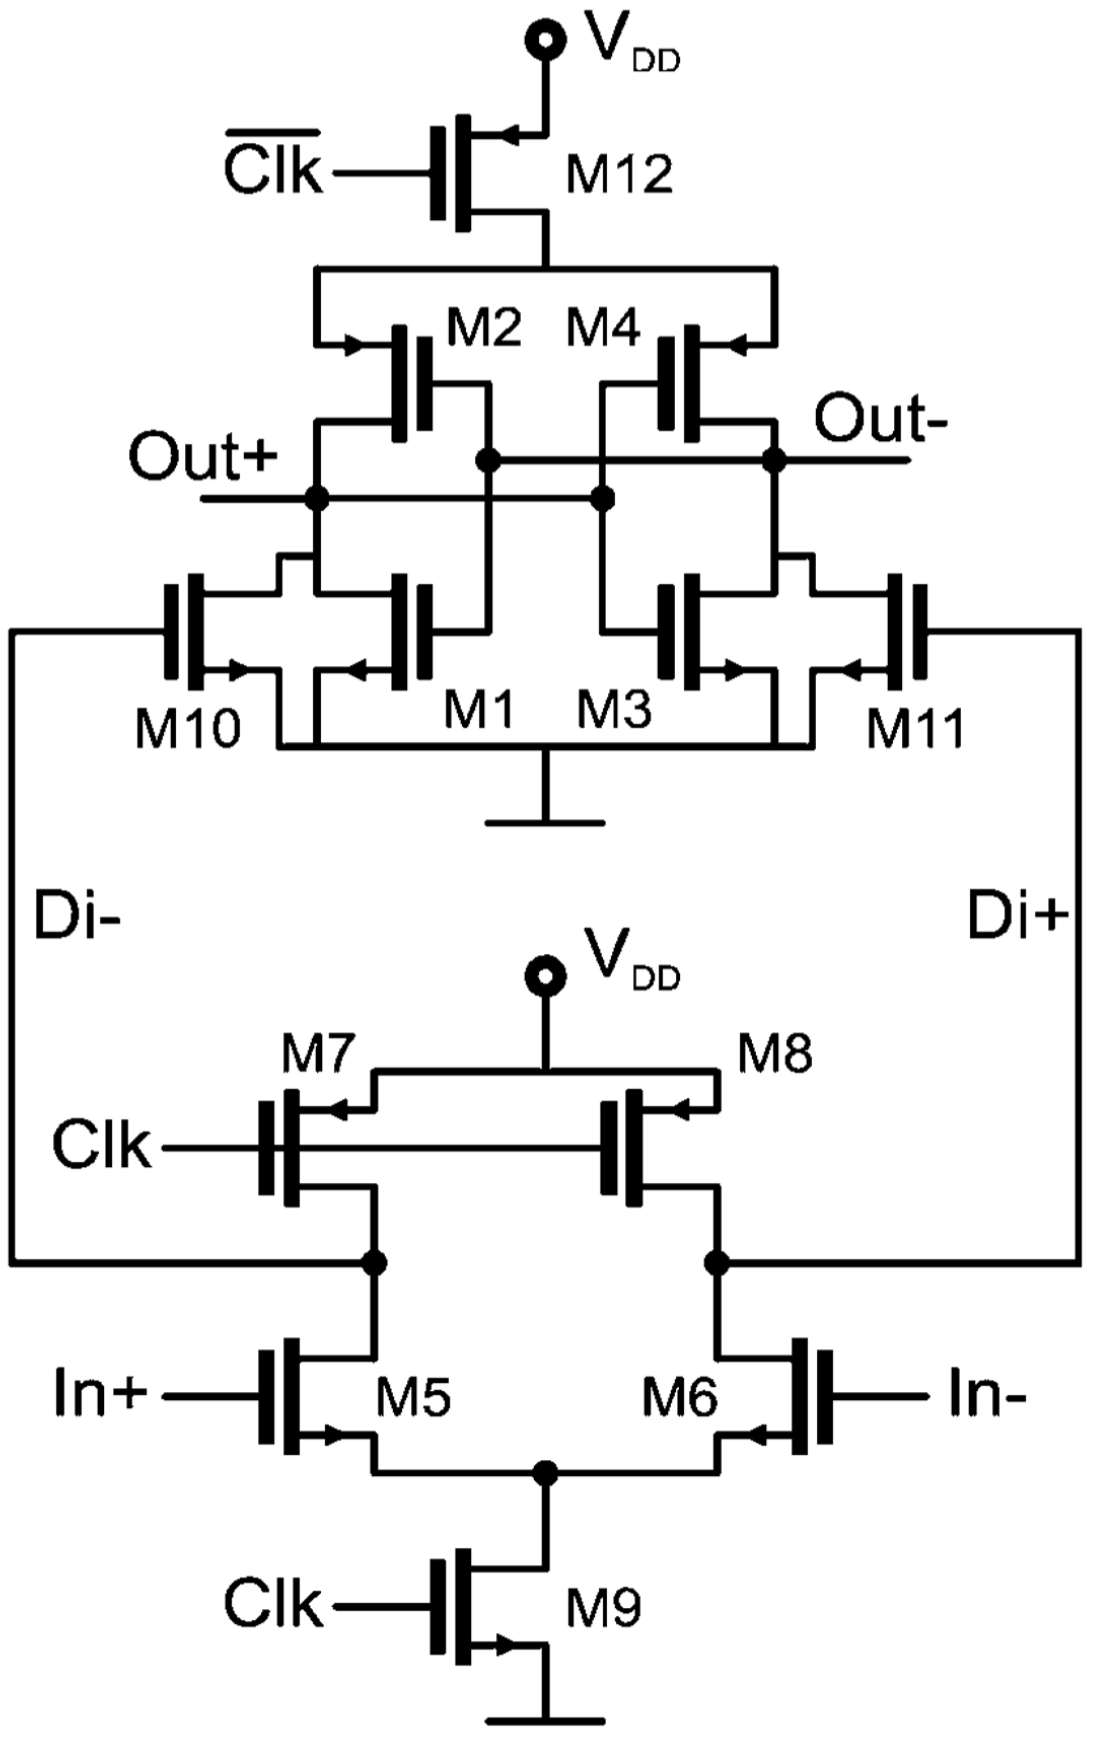
\includegraphics[width=0.6\linewidth]{Figures/Rep2DoubleTail.png}
	\caption{Double tail sense amplifier, Source: \cite{schinkel2009low}.} 
    \label{fig:rep2:doubletail}
\end{figure}

A sense amplifier is not only samples incoming data fast, it also realigns it to a clock and regenerates the voltage.
The improved sense amplifier is based on the \textit{double-tail} amplifier (see: \cref{fig:rep2:doubletail}, \cite{schinkel2007double}).
The upper-tail shows the latching stage and the lower-tail shows the input stage.
There is no need for dedicated reset transistors.
This topology has an extra degree of freedom because it enables optimization between speed, offset, power and common-mode voltage.

The offset is the bottleneck for the amplifier.
The transistor dimensions are optimized to get the lowest offset standard deviation per unit of power cost.

The influence of the change in technology (Dennard scaling) on the optimum swing is not present.
The $C_{wire}/length$ does not change significantly over different technologies

% The sense amplifier is able to quickly recover the the voltage to full swing and also samples incoming data .
% the improved sense amplifier which can also operate over a wide common-mode and supply voltage range.


\subsubsection{Transceiver} \label{sss:rep2:transceiver}
The source-synchronous scheme is most likely to be used in combination with the transmitter (see: \cref{fig:rep2:transceiver}).
Parallel to the capacitive transmitter a half-rate clock is transmitted ("double-data rate").
The sense amplifier consist of two parts (as earlier described).


\begin{figure}[]
	\centering
	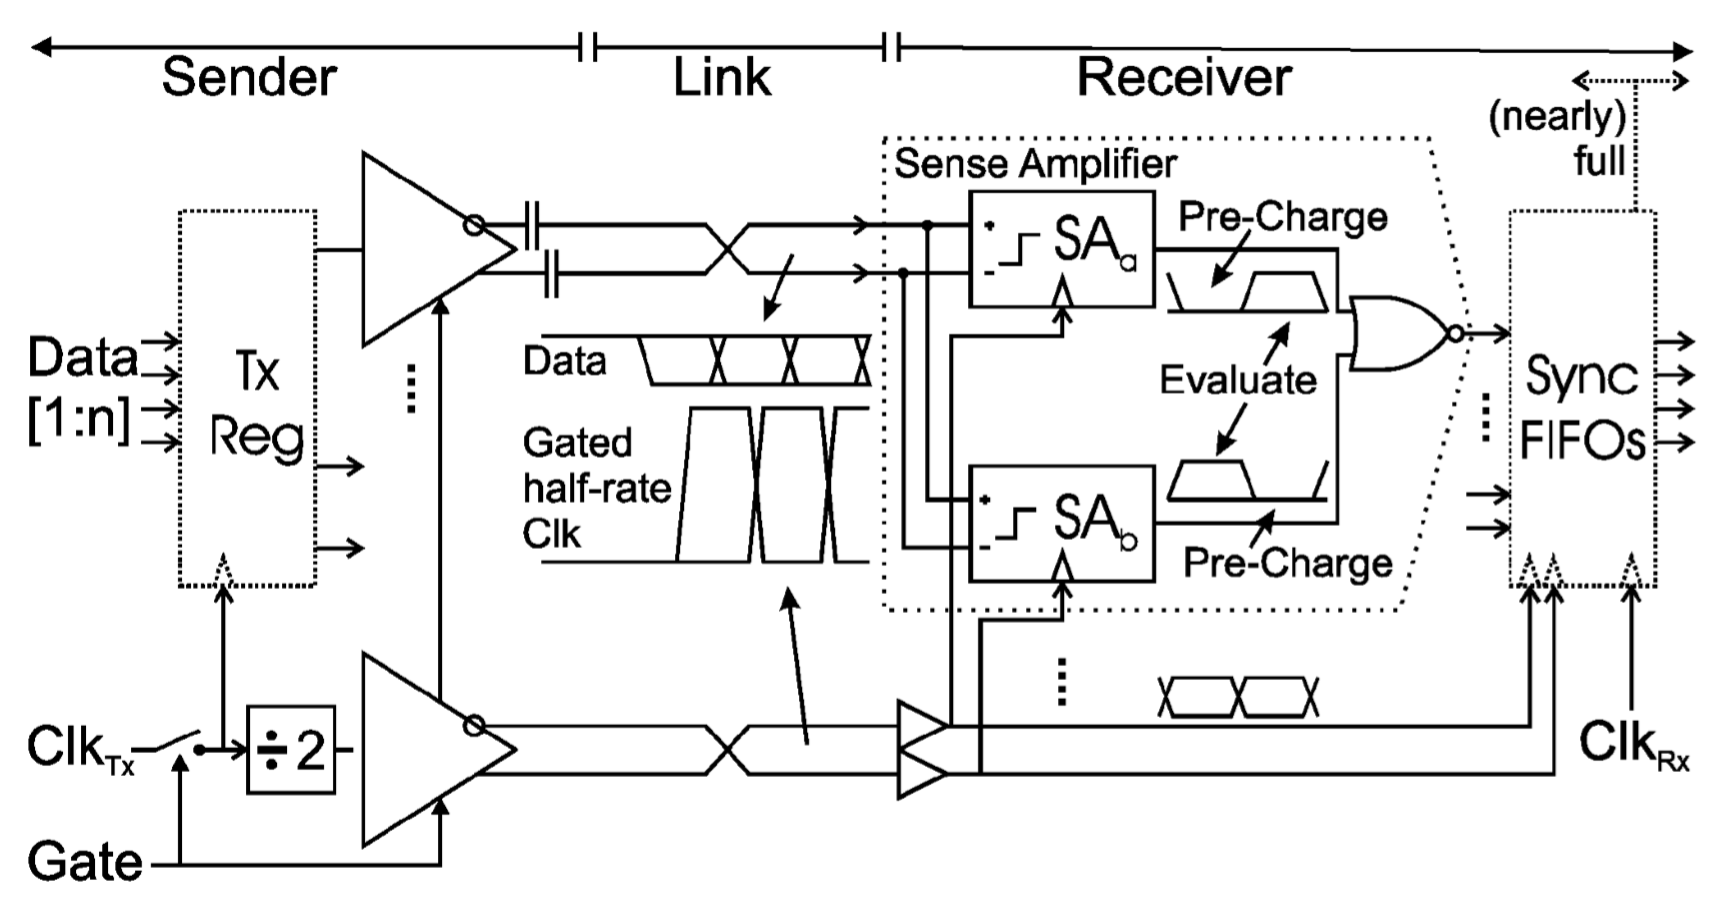
\includegraphics[width=0.9\linewidth]{Figures/Rep2Transceiver.png}
	\caption{The complete transceiver, Source: \cite{schinkel2009low}.} 
    \label{fig:rep2:transceiver}
\end{figure}

%Cascaded Transceivers

In certain routing schemes, intermediate routers can be ommitted by using direct forwarding (wave-pipeling).
To test this concept a number of cascaded transceivers were simulated.
The startup of the clock appears to be a speed-limiting factor.
Clock-wires in a two times larger metal layer (four times lower resistance) show that the system is capable to run at $9 Gb/s$.
Without this optimization it is still possible to reach $5 Gb/s$.
To test the effect of crosstalk a simulation with a bus was doen.
Almost no crosstalk was visible in the output of three neighbouring channels.

%Conclusion
The combination of a low-swing capacitive pre-emphasis transmitter, a twisted differential wires bus, a double-tail sense amplifier and a source-synchronous clocking is very suitable for communication in a NoC.
The circuits are compatible with standard CMOS circuits and scalable for future technologies.

%%%%%%%%%%%%%%%%%%%%%%%%%%%  3  %%%%%%%%%%%%%%%%%%%%%%%%%%% 
\subsection{High performance on-chip differential signaling using passive compensation for global communication \cite{zhang2009high}} \label{ss:zhang2009high}
%%%%%%%%%%%%%%%%%%%%%%%%%%%  3  %%%%%%%%%%%%%%%%%%%%%%%%%%% 

\begin{figure}	\centering
	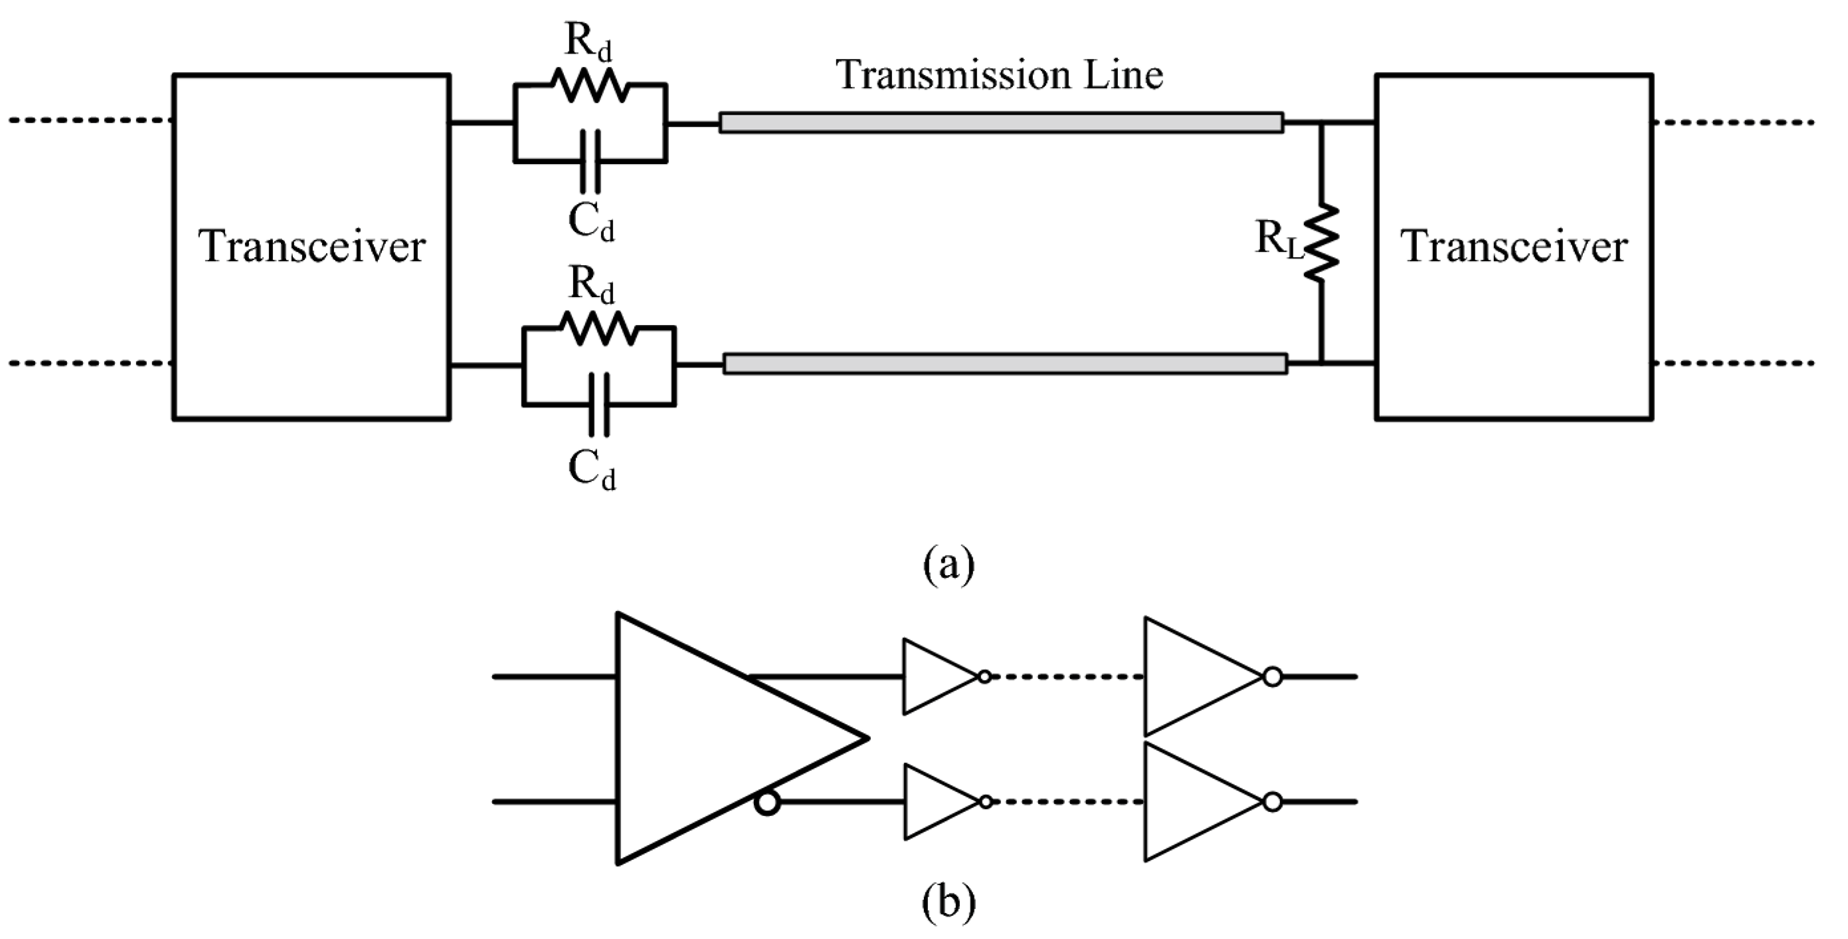
\includegraphics[width=0.95\linewidth]{Figures/Rep3Overview.png}
	\caption{Proposed signaling schema for global wiring: (a) one stage structure; (b) Sense Amplifier + inverter chain structure, Source: \cite{zhang2009high}.} 
    \label{fig:rep3:overview}
\end{figure}

The interconnect of a chip is regarded one of the most critical factors in the determination of performance and power consumption according the ITRS (International Technology Roadmap for Semiconductor) roadmap.
% MISSCHIEN ZIN VERANDEREN DIRECT OVERGENOMEN
For instance, the \textit{1 mm} global RC wire delay (at 45 \textit{nm} technology) is 385 \textit{ps} while the 10 level FO4 delay is below 200 \textit{ps}.
Traditionally the interconnect delay problem is dealed with by implementing a buffer (\textit{buffer insertion} also known as \textit{repeated RC wires}).
However, this introduces a power overhead, i.e. approximately half of the dynamic power is dissipated by the repeaters.

\motive
The use of \accs{otl} deliver signals with speed of light and consumes less power than repeaters, but the \acc{isi} can be a problem for performance.

\objective
A high performance on-chip global signaling with passive compensation is proposed (see \cref{fig:rep3:overview}).
The design is covered and an optimization flow is proposed that optimizes the scheme for a given technology and wire dimension.
Finally the \ac{otl} is compared with repeated RC wires.

\summary
%A. On-Chip T-Line
The proposed signaling schema for global wiring is shown in \cref{fig:rep3:overview}.
For a wire the values of $R_{d}, C_{d} and R_{l}$ determine the eye-opening which are optimized in the optimization flow.

The \ac{otl} is very lossy ($R \neq 0$ and $G \neq 0$) because of the miniaturization of the cross section of the wire.
It can operate in the RC or in the LC region given different frequencies (respectively based on $\omega L \ll R$ (upto 10 GHz) and $\omega L \gg R$).
In LC region the phase velocity and attenuation are independent of frequency.

\begin{figure}	\centering
	
	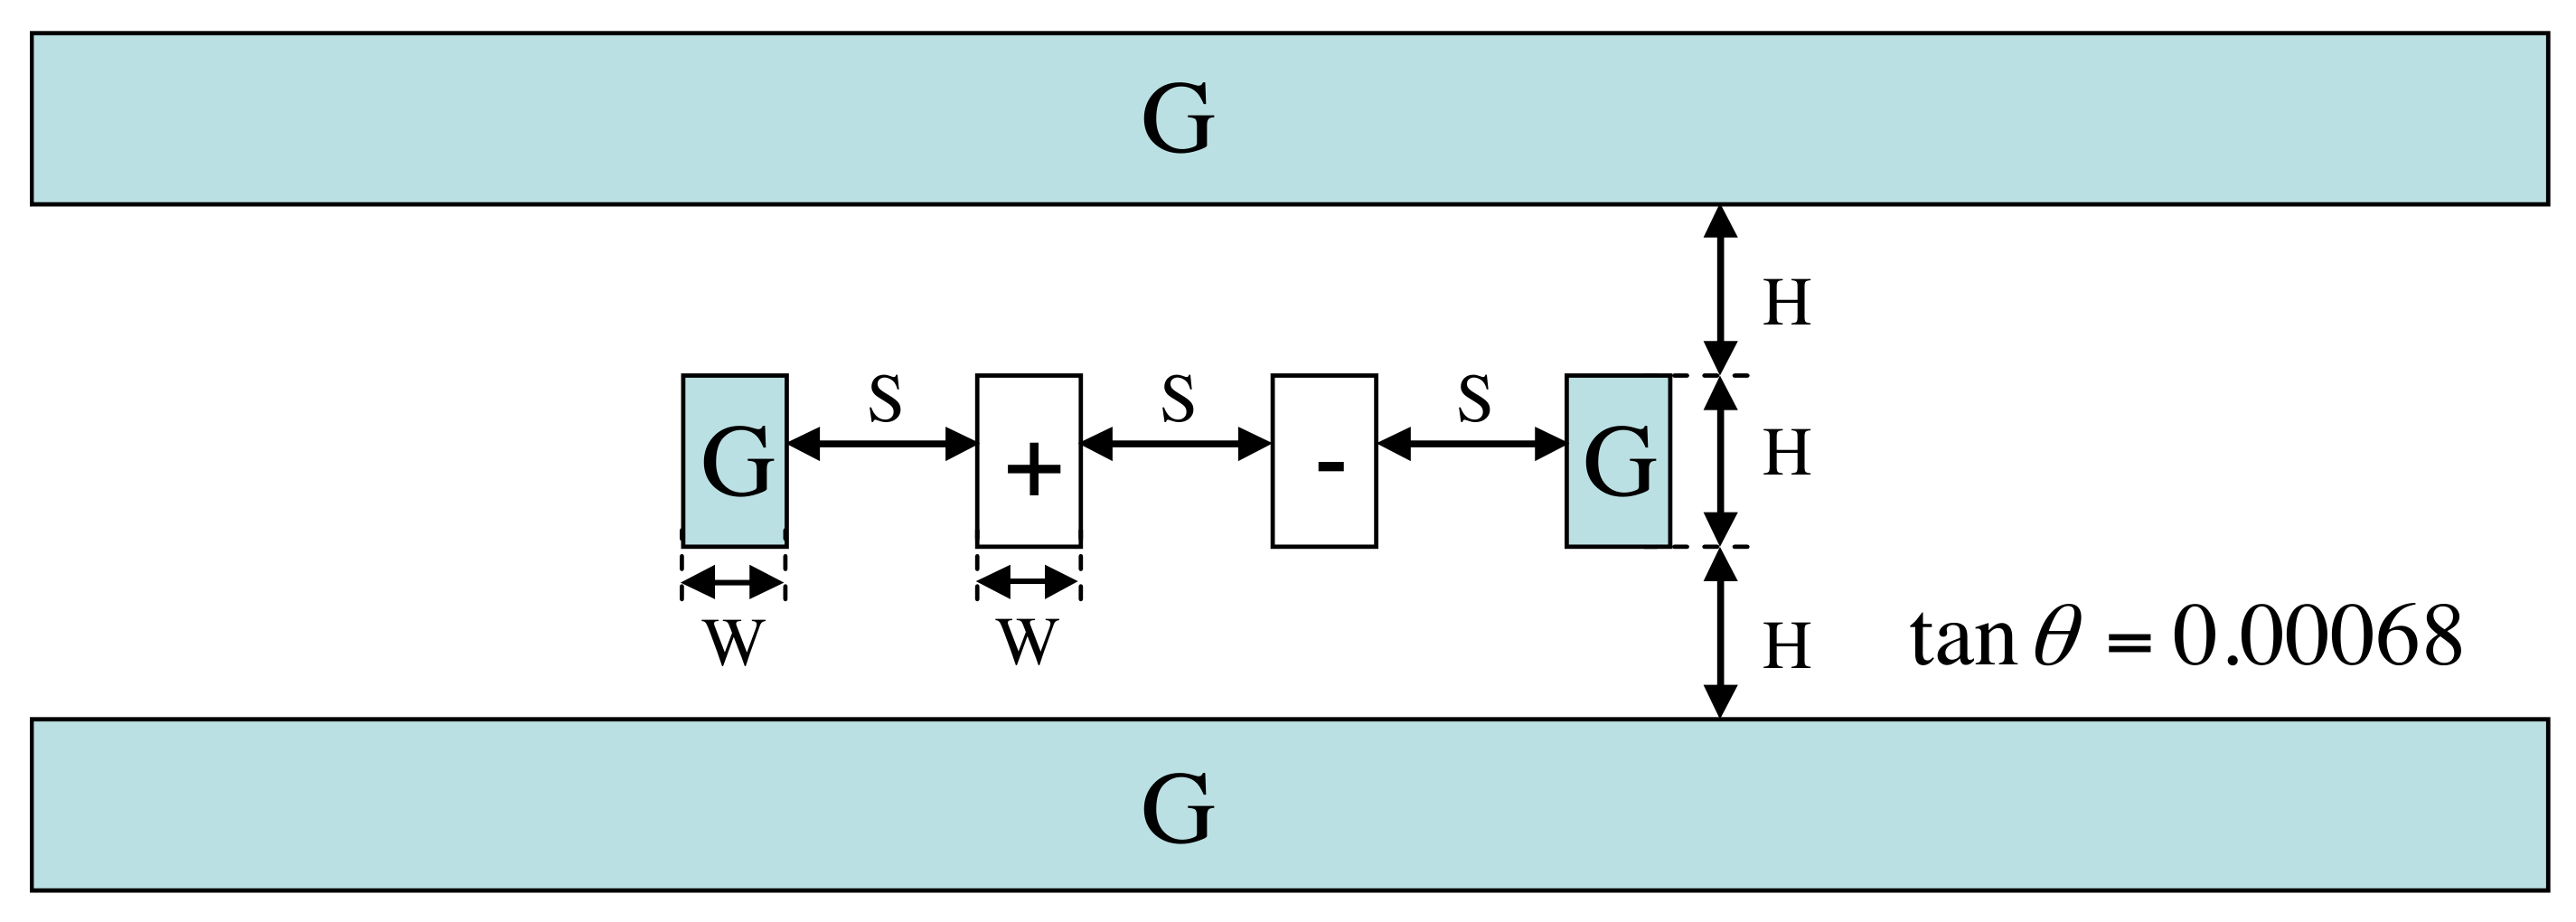
\includegraphics[width=0.95\linewidth]{Figures/Rep3TransmissionLine.png}
	\caption{Cross section of a differential stripline, Source: \cite{zhang2009high}.} 
    \label{fig:rep3:crosssection}
\end{figure}
% Transmission line geometries:
% The length of the global communication in this paper is set to \textit{5 mm}.
According the ITRS roadmap the wire thickness and width ratio should be 2 (see: \cref{fig:rep3:crosssection}).
Larger spacings (S) let the characteristic impedance ($Z_{0}$) increase, which reduces the attenuation and hence gives better eye-diagram performance. %3) Delay and power models ==>> NOT WRITTEN ANYTHING, DO NOT SEE THE USE
% The spacing is varied so that $S = 0.5H, H, 1.5H and 2H$

% B. Transceiver design and modeling
The transceiver stage sense amplifier is based on the same sense amplifier as in \cref{ss:schinkel2009low}.
This design is chosen due to its flexibility to balance the performance metrics.
Simulations have shown that the termination resistance ($R_{l}$) and ($R_{d}$) are dominant in the power consumption.

%Problem formulation and optimization flow
To find the optimum passive compensation for high speed compensation four parameters are optimized: $R_{l}$, $R_{d}$, $C_{d}$ and $R_{s}$.
Here $R_{s}$ is the output resistance of the inverter chain output.
It has to be optimized to minimize the sense amplifier delay.

This optimization problem is constrained as a non-linear programming problem and uses the \acc{sqp} to solve it.
The global design goals are to minimize: latency (\textbf{min-d}), latency-power product (\textbf{min-dp}) and the $latency^{2}$-power product (\textbf{min-ddp}).
% global explanation of optimizaiton work flow
The optimization flow inputs are the technology node and wire dimensions.
Then the wire and transceiver model are build respectively.
In each iteration the delay and power parameters of the wire are derived after which the step response of the T-line is simulated.
Based on this the eye opening is determined.
Given the design goals the cost function is evaluated by combination of delay and power of both wires and transceivers.
This is utilized by the \ac{sqp} algorithm for optimization.
Finally, the flow output the optimal values.

% Experimental results
The scheme is optimized under the aforementioned design goals and with four different spacing and then compared with repated RC wires (which are also optimized for the different design goals).

For comparison purposes the normalised delay, power and throughput are used which are respectively defined as: $delay_{n} = \frac{\text{propagation delay}}{\text{wire length}}$, $power_{n} = \frac{\text{energy per bit}}{\text{wire length}}$ and $throughput_{n} = \frac{\text{frequency}}{\text{wire pitch}}$.

\begin{figure}	\centering
	
	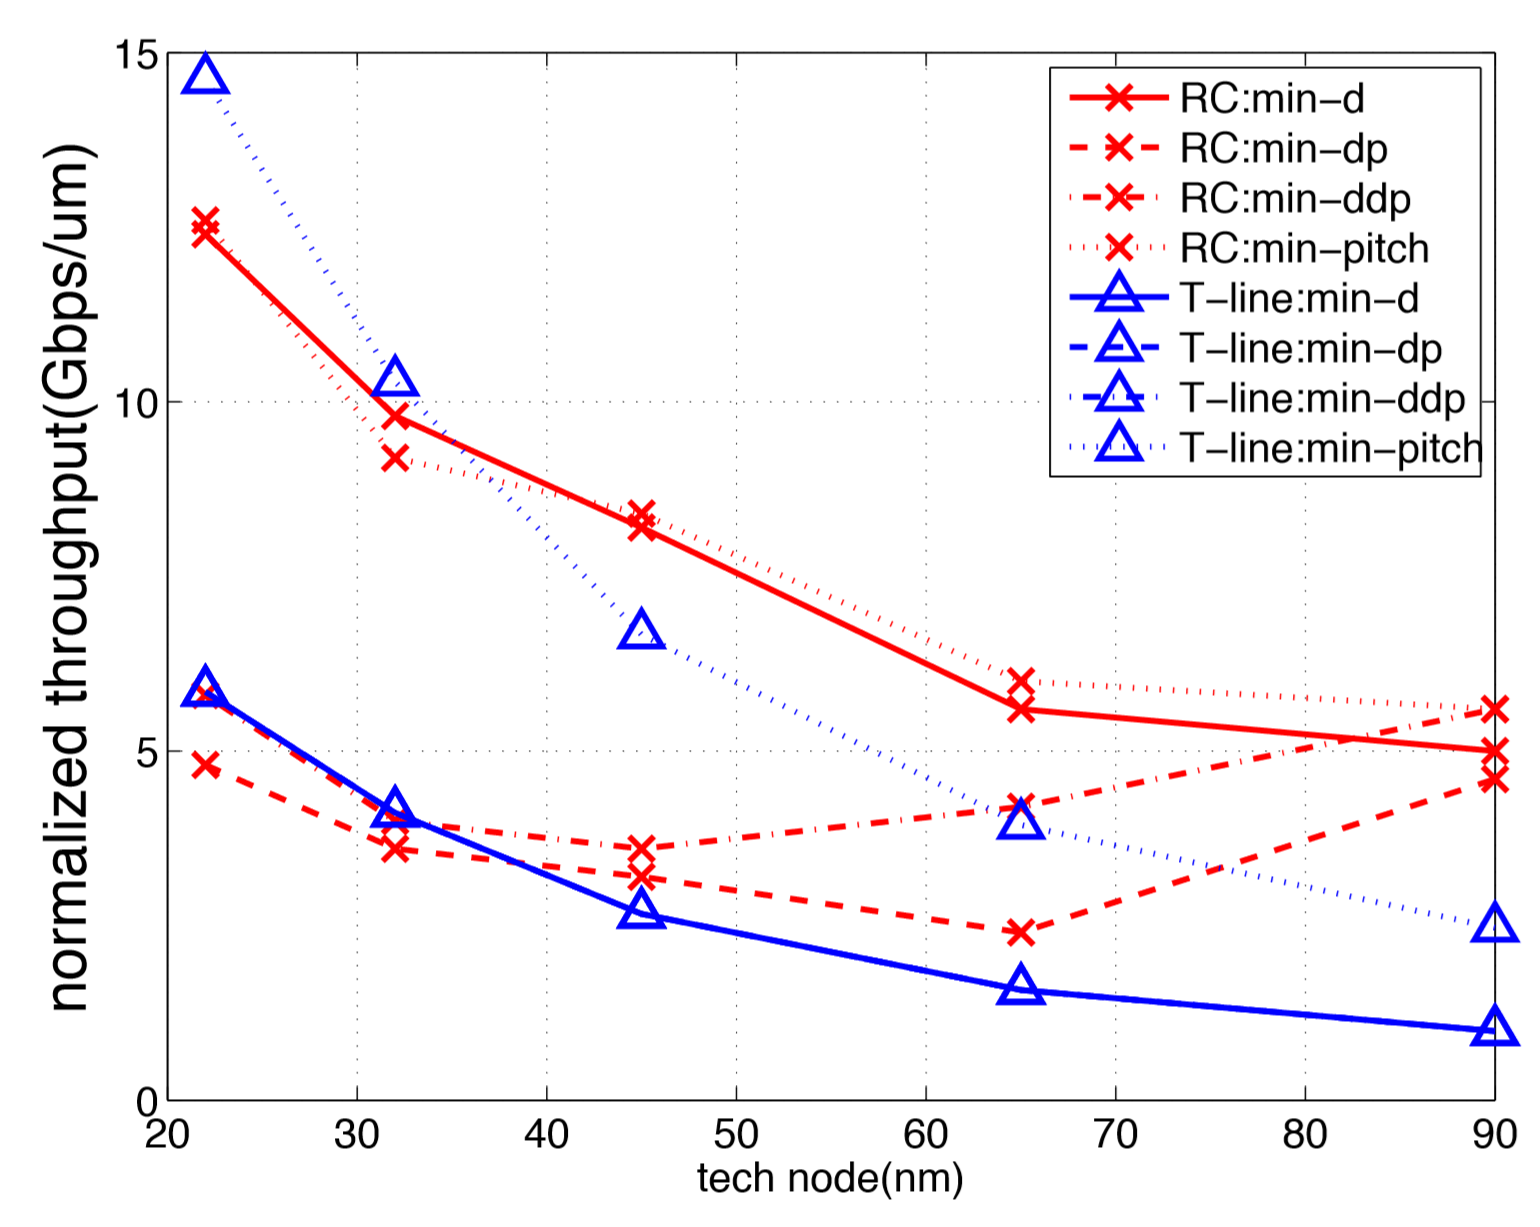
\includegraphics[width=0.95\linewidth]{Figures/Rep3NormThrough.png}
	\caption{Normalized throughput between repeated RC wire and on-chip T-line, Source: \cite{zhang2009high}.} 
    \label{fig:rep3:normthrough}
\end{figure}

The $delay_{n}$ and $power_{n}$ of  \ac{otl} are much better than the RC wire. For $delay_{n}$ from the 60 nm technology node the \ac{otl} performs better.
For $power_{n}$ the \ac{otl} performs better in the whole technology node spectrum.
In \cref{fig:rep3:normthrough} the $throughput_{n}$ is shown with regards to the different optimization criteria.
At \textit{90 nm} technology the RC wire has higher throughput than the \ac{otl}.
The throughput of RC wires decreases due to the usage of smaller repeaters and smaller wire width to reduce the power in the range from \textit{90 nm} to \textit{45 nm}.
In general after the \textit{45 nm} technology the throughput of the schemes are very close, but the throughput of the \ac{otl} is higher.

%conclusion
The wire with the largest spacing (S=2H) give the optimal results, this is due to higher $Z_{0}$ with reduces the attenuation along the wire.


\section{Comparison}
\section{Conclusion} \label{sec:conclusion}


% Conclusions and future prospects
% are clearly linked to the research question in the introduction, indicating to what extent the research question has been answered
% follow logically from all the previous material 
% are preferably followed by recommendations for further research (future prospects)word limit is respected (+/- 200)

% In the conclusion, you should:

% - Summarize major contributions of significant studies and articles to the body of knowledge under review, maintaining the focus established in the introduction.
% - Evaluate the current "state of the art" for the body of knowledge reviewed, pointing out major methodological flaws or gaps in research, inconsistencies in theory and findings, and areas or issues pertinent to future study.
% - Conclude by providing some insight into the relationship between the central topic of the literature review and a larger area of study such as a discipline, a scientific endeavor, or a profession.

\section{Remarks}
From \cite{agrawal20098} the importance of the \ac{pll} and the \ac{dll} was grasped. 
This is a subject that could be engaged more in the lecture slides of this course.
The paper from \cite{agrawal20098} was pleasant to review but relatively hard to summarize without diving into too much details.

\bibliographystyle{ieeetr}
\bibliography{biblio}

\end{document}
